% Research report of studies/oran_baseline
% Build: run `latexmk` in this directory (.latexmkrc selects pdflatex), or `pdflatex main.tex` twice.
% Figures of E1-E3 are regenerated with English labels by make_figures.py (see Appendix B).
\documentclass[11pt,a4paper]{article}

\usepackage[T1]{fontenc}
\usepackage{lmodern}
\usepackage{microtype}
\DisableLigatures[-]{encoding = T1, family = tt*}   % keep "--option" from turning into an en dash
\usepackage[margin=2.3cm]{geometry}
\usepackage{amsmath,amssymb}
\usepackage{graphicx}
\usepackage{booktabs,tabularx,multirow,array}
\usepackage{caption}
\usepackage{float}
\usepackage{enumitem}
\usepackage{xcolor}
\usepackage{listings}
\usepackage{tikz}
\usetikzlibrary{positioning,arrows.meta,calc,decorations.pathreplacing}
\usepackage[hidelinks]{hyperref}

\captionsetup{font=small,labelfont=bf}
\setlist{itemsep=2pt,topsep=4pt}
\renewcommand{\arraystretch}{1.15}
\newcolumntype{Y}{>{\raggedright\arraybackslash}X}
\newcolumntype{P}[1]{>{\raggedright\arraybackslash}p{#1}}
\usepackage{url}
\DeclareUrlCommand\codeurl{\urlstyle{tt}}   % monospace names that may break after _ / . -
\DeclareRobustCommand{\code}[1]{\codeurl{#1}}  % robust wrapper so it also works in captions
\makeatletter\g@addto@macro\UrlBreaks{\do\_\do\-}\makeatother
\newcommand{\dB}{\,dB}
\newcommand{\Gbps}{\,Gbit/s}
\setlength{\parskip}{3pt}

\lstset{basicstyle=\ttfamily\footnotesize, breaklines=true, columns=fullflexible,
        frame=single, rulecolor=\color{gray!50}, backgroundcolor=\color{gray!5},
        xleftmargin=2pt, xrightmargin=2pt}

\title{Baseline Study of the O-RAN 7.2x Simulator\\[6pt]
  \large Cat A / Cat B, Fronthaul IQ Compression, Ray-Traced Closed Loop,\\
  and Fronthaul Load of Lower-Layer Splits in Cell-Free MIMO}
\author{Research direction \code{studies/oran_baseline}}
\date{6 November 2026\\[2pt]\small Experiments run on 4--5 October 2026 and 5 November 2026 (F1)}

\begin{document}
\maketitle

\begin{abstract}
This report documents all work in the \code{studies/oran_baseline} direction. The direction had two goals: to verify that
the in-house O-RAN 7.2x downlink link-level simulator (\code{oran/}, built on Sionna 2.2) behaves correctly and consistently,
and to fix the baseline settings that the later research directions reuse. The report first describes the simulator's
signal chain, the four lower-layer functional splits (3GPP option 7-1, O-RAN 7.2x Cat A and Cat B, option 8), the O-RAN
fronthaul compression methods, the fronthaul load model and the closed-loop link adaptation. It then gives the setup, results
and analysis of four sets of experiments. Main findings:
\begin{enumerate}[leftmargin=*]
  \item With an ideal fronthaul, the BLER curves of Cat A and Cat B coincide exactly (both need 23.10\dB for BLER $=0.1$ at MCS 20,
        256QAM). This confirms that the two signal paths produce bit-identical air-interface signals. With the same compression,
        Cat B needs about half the fronthaul rate of Cat A (4 layers instead of 8 antennas).
  \item Block floating point (BFP) at 9 and 7 bit is practically lossless ($\le 0.06$\dB); 6 bit starts to cost; \textbf{5 bit is
        the breaking point}. With two-user MU-MIMO, Cat A hits an error floor near BLER 0.21 and Cat B loses 0.87\dB. At equal
        bit width, block scaling gives 2.0--5.6\dB more SQNR than BFP.
  \item In the closed loop, \textbf{the CSI-IM never sees compression distortion}. With one user the CSI-RS hardly sees it either;
        with two users the NZP-IMR captures only 30--45\% of the SINR drop on the data slots. The rest can only be absorbed by
        outer-loop link adaptation (OLLA) from ACK/NACK feedback.
  \item In cell-free MIMO (4 O-RUs $\times$ 8 TX, 4 UEs), the lowest fronthaul load that keeps at least 99\% of the ideal-fronthaul
        throughput (100\,MHz, sum of 4 links) is 48.8\Gbps for option 7-1, 45.2\Gbps for Cat A, 11.7\Gbps for Cat B with
        modulation compression, and 65.1\Gbps for option 8. Cat B with modulation compression needs about a quarter of the
        load of the other splits, with no throughput loss.
\end{enumerate}
\end{abstract}

\tableofcontents
\newpage

% =====================================================================
\section{Background and goals}
% =====================================================================

\subsection{Background}

O-RAN splits the gNB physical layer in two: the High-PHY runs in the O-DU and the Low-PHY in the O-RU; the interface between
them is the fronthaul. The O-RAN WG4 CUS specification uses split 7.2x, which comes in two categories depending on where
precoding happens:
\begin{itemize}
  \item \textbf{Category A}: precoding in the O-DU; the fronthaul carries frequency-domain IQ per antenna (antenna port);
  \item \textbf{Category B}: precoding in the O-RU; the fronthaul carries frequency-domain IQ per layer, and the precoding weights
        are sent in the C-plane.
\end{itemize}
Fronthaul bandwidth grows linearly with the number of antennas, the bandwidth and the IQ bit width. It is one of the main
bottlenecks of massive MIMO and of cell-free (distributed) MIMO. Annex A of the O-RAN specification defines IQ compression
methods (block floating point, block scaling, $\mu$-law, modulation compression) that reduce the load at the price of
quantization distortion. 3GPP also defines option 7-1 (frequency-domain IQ of the whole carrier) and option 8 (time-domain
samples, i.e.\ classic CPRI), which serve as references here.

\code{oran/} in this repository is a downlink PDSCH link-level simulator built on NVIDIA Sionna 2.2 (PyTorch). The same link
can be switched between the four splits and the compression methods, and it supports two closed-loop modes: ray tracing
(Sionna RT) and random drops in the TR 38.901 UMi model. Before using it in the later directions (\code{csirs_du_ru},
\code{srsbf}, \code{twin_ci_compression}, \code{dynamic_split}), we needed to confirm that it behaves sensibly and to agree on
common baseline settings. That is the purpose of this direction.

\subsection{Questions}

\begin{description}[leftmargin=1.2em, style=nextline]
  \item[Q1 (open loop)] At a fixed MCS, how do the BLER and EVM of Cat A and Cat B depend on the IQ compression bit width and
        the SNR? How much do BFP, block scaling and $\mu$-law differ?
  \item[Q2 (closed loop)] In a ray-traced closed loop (CSI-RS $\to$ CQI $\to$ MCS + OLLA), how much of the compression
        distortion is visible to the CSI-RS measurement, and how much can only be absorbed by OLLA?
  \item[Q3 (cell-free, F1)] In a cell-free downlink with TR 38.901 UMi drops, what fronthaul load do option 7-1, 7.2x Cat A,
        7.2x Cat B and option 8 need with their respective compression schemes? With MCS selection by CQI table lookup,
        which compression settings cost no throughput?
\end{description}

\subsection{Experiments}

Table~\ref{tab:overview} lists the experiments. E1--E3 ran on a server with two Tesla T4 GPUs; F1 ran on a T4.

\begin{table}[H]
\centering
\caption{Experiments. All result directories are under \code{results/} in the repository root (not tracked by git).}
\label{tab:overview}
\footnotesize
\begin{tabularx}{\textwidth}{@{}l l l l Y l@{}}
\toprule
ID & Date & Script & Channel & Content & Result directories \\
\midrule
E1  & 10-04 & \code{compare_cat_a_b.py} & CDL-C & Cat A/B $\times$ BFP width $\times$ SNR (open loop) & \code{cat_a}, \code{cat_b}, \code{cat_ab} \\
E1$'$ & 10-04 & \code{compare_cat_a_b.py} & CDL-C & BFP vs block scaling vs $\mu$-law (open loop) & \code{methods_a}, \code{methods_b}, \code{methods} \\
E2  & 10-05 & \code{rt_closed_loop.py} & ray tracing & Closed-loop baseline, SU (1 UE) and MU (2 UEs) & \code{rt_su}, \code{rt_mu} \\
E3  & 10-05 & \code{rt_compare_compression.py} & ray tracing & Visibility of compression distortion in the closed loop (paired drops) & \code{csi_su*}, \code{csi_mu*} \\
F1  & 11-05 & \code{split_fronthaul_load.ipynb} & UMi drops & Fronthaul load and throughput of four splits $\times$ compression, cell-free & \code{split_fronthaul_load_20261105/} \\
\bottomrule
\end{tabularx}
\end{table}

In addition, \code{closed_loop_walkthrough.ipynb} steps through one closed-loop simulation module by module
(Appendix~\ref{sec:walkthrough}). It is meant for understanding the code and is not a source of statistical conclusions.

% =====================================================================
\section{Simulator and system model}
% =====================================================================

\subsection{Scope and specifications}

Only the physical layer is simulated: from the transport block (TB) handed down by the MAC over FAPI to the CRC check at the
UE. RRC, PDCP, RLC and MAC are not simulated; they appear only as configuration parameters (MCS, number of layers, RNTI, DMRS
ports, \ldots), and the information bits are random. The implementation follows TS 38.211 V18.6.0, TS 38.212 V18.5.0,
TS 38.214 V18.2.0 (Rel-18) and O-RAN WG4 CUS v22.00. Software: Sionna 2.2.0 (PHY, SYS, RT), PyTorch 2.14.1 with CUDA 12.6,
Python 3.12.

The downlink processing chain is:
\begin{description}[leftmargin=1.2em, style=nextline]
  \item[O-DU (High-PHY)] TB CRC $\to$ code-block segmentation + CB CRC $\to$ LDPC encoding $\to$ rate matching $\to$ scrambling
        $\to$ QAM mapping $\to$ layer mapping $\to$ RE mapping (data + DMRS) $\to$ [Cat A / 7-1 / 8: precoding]
        $\to$ [option 8: IFFT + CP];
  \item[Fronthaul] 16-bit fixed point $\to$ per-PRB compression $\to$ (transport) $\to$ decompression; for Cat B, the weights are
        additionally compressed per PRB bundle and sent in the C-plane (Section Extension 11);
  \item[O-RU (Low-PHY)] [Cat B: per-RE precoding with the received weights] $\to$ IFFT + CP (not for option 8) $\to$ RF
        (a DAC hook is provided);
  \item[Channel] one independent link per (UE, O-RU) pair (CDL, ray tracing or UMi) + AWGN;
  \item[UE] CP removal + FFT $\to$ DMRS channel estimation $\to$ LMMSE equalization $\to$ soft demapping $\to$ layer demapping
        $\to$ descrambling / rate recovery / LDPC decoding $\to$ CRC.
\end{description}

Figure~\ref{fig:splits} marks where each split cuts this chain.

\begin{figure}[H]
\centering
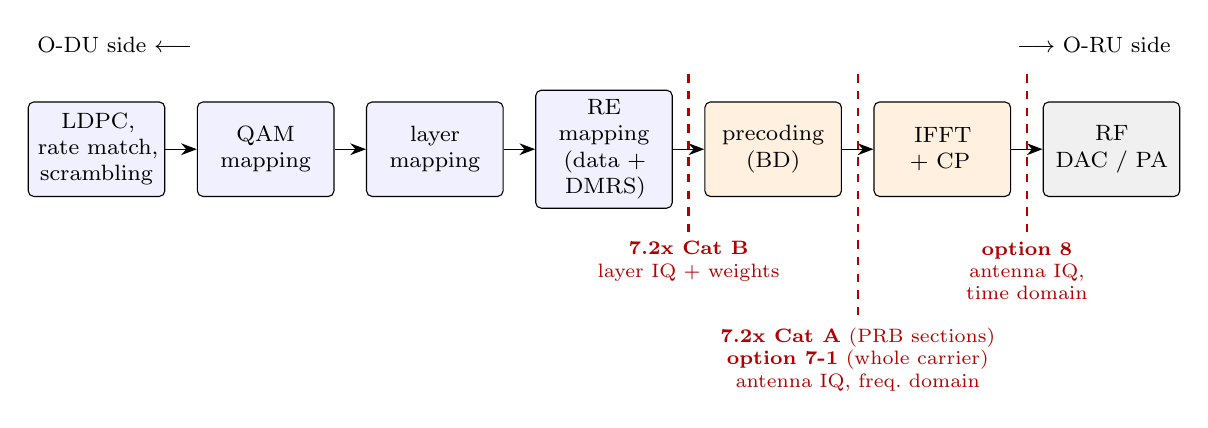
\begin{tikzpicture}[
    >={Stealth[length=2mm]}, node distance=4mm,
    blk/.style={draw, rounded corners=2pt, minimum height=12mm, text width=15mm, align=center,
                font=\footnotesize, fill=#1},
    blk/.default=white]
  \node[blk=blue!6]                (enc)  {LDPC,\\rate match,\\scrambling};
  \node[blk=blue!6, right=of enc]  (mod)  {QAM\\mapping};
  \node[blk=blue!6, right=of mod]  (lay)  {layer\\mapping};
  \node[blk=blue!6, right=of lay]  (re)   {RE mapping\\(data +\\DMRS)};
  \node[blk=orange!12, right=of re]   (pre)  {precoding\\(BD)};
  \node[blk=orange!12, right=of pre]  (ifft) {IFFT\\+ CP};
  \node[blk=gray!12, right=of ifft]   (rf)   {RF\\DAC / PA};
  \foreach \a/\b in {enc/mod, mod/lay, lay/re, re/pre, pre/ifft, ifft/rf}
    \draw[->] (\a) -- (\b);
  \foreach \a/\b/\y/\lab in {
      re/pre/-1.05/{\textbf{7.2x Cat B}\\layer IQ + weights},
      pre/ifft/-2.15/{\textbf{7.2x Cat A} (PRB sections)\\\textbf{option 7-1} (whole carrier)\\antenna IQ, freq.\ domain},
      ifft/rf/-1.05/{\textbf{option 8}\\antenna IQ,\\time domain}} {
    \coordinate (m) at ($(\a.east)!0.5!(\b.west)$);
    \draw[dashed, thick, red!70!black] ($(m)+(0,0.95)$) -- ($(m)+(0,\y)$);
    \node[font=\scriptsize, align=center, below, red!70!black] at ($(m)+(0,\y)$) {\lab};
  }
  \node[font=\footnotesize, above=5mm of enc.north west, anchor=south west] {O-DU side $\longleftarrow$};
  \node[font=\footnotesize, above=5mm of rf.north east, anchor=south east] {$\longrightarrow$ O-RU side};
\end{tikzpicture}
\caption{Downlink physical-layer chain and the position of the four splits. For each red dashed line, the functions on the
left run in the O-DU and those on the right in the O-RU; the text below says what the fronthaul carries. Option 7-1 and
Cat A cut at the same place and differ only in the interface: 7-1 always streams the whole carrier, with no sections, no
O-RAN compression and no C-plane.}
\label{fig:splits}
\end{figure}

\subsection{The four functional splits}

Table~\ref{tab:splits} compares the four splits. \textbf{Without compression, all four put bit-identical signals on the
antennas} (verified by unit tests). All differences between them in this report therefore come from what the fronthaul
carries and how it is quantized.

\begin{table}[H]
\centering
\caption{The four functional splits (\code{ORANConfig.category})}
\label{tab:splits}
\footnotesize
\begin{tabularx}{\textwidth}{@{}P{1.6cm} P{2.4cm} Y P{2.3cm} P{2.9cm}@{}}
\toprule
Split & Reference & Fronthaul carries (per O-RU link) & O-RU does & Compression here \\
\midrule
option 7-1 \newline \code{"7-1"} & TR 38.801 \S 11.1.2.7, TR 38.816 \S 4.2 / Annex A
  & frequency-domain IQ of every antenna, \textbf{whole carrier, every symbol}, independent of scheduling; no C-plane
  & IFFT + CP & none standardized; uniform fixed point, $w$ bit per I/Q \\
7.2x Cat A \newline \code{"A"} & O-RAN CUS v22 \S 4.2
  & frequency-domain IQ of every antenna, only PRBs that carry data (sections), plus C-plane section descriptions
  & decompression, IFFT + CP & BFP / block scaling / $\mu$-law (Annex A.1--A.3) \\
7.2x Cat B \newline \code{"B"} & O-RAN CUS v22 \S 4.2
  & frequency-domain IQ of every layer, plus precoding weights in the C-plane (SE 11)
  & per-RE precoding, IFFT + CP & as Cat A, or modulation compression (Annex A.5) \\
option 8 \newline \code{"8"} & TR 38.801 \S 11.1.2.8
  & time-domain samples of every antenna (incl.\ guard band and CP); no C-plane
  & RF only & none standardized (CPRI); uniform fixed point, $w$ bit per I/Q \\
\bottomrule
\end{tabularx}
\end{table}

Where the compression distortion enters the chain determines how it affects the receivers. This is the key to all results
below (Table~\ref{tab:inject}).

\begin{table}[H]
\centering
\caption{Where fronthaul compression distortion enters, and what it does}
\label{tab:inject}
\footnotesize
\begin{tabularx}{\textwidth}{@{}P{2.7cm} Y Y@{}}
\toprule
Source & Effect on the PDSCH & Visible on CSI-RS / CSI-IM? \\
\midrule
Cat A / 7-1 U-plane (antenna domain)
  & spatially white noise on the antennas, power proportional to the sum of all UE signals on that RE; not precoded, so BD
    cannot null it: self-distortion plus leakage to the co-scheduled UE
  & partly: the distortion of the co-scheduled UE's CSI-RS leaks into this UE and is measured on the NZP-IMR; self-distortion
    only shows up as CMR channel-estimation error \\
Cat B U-plane (layer domain)
  & layer-domain noise is beamformed with this UE's weights and nulled at the co-scheduled UE by BD: self-distortion only,
    but it gets the same array gain as the signal
  & essentially no: it only shows up as CMR channel-estimation error \\
Cat B weights (C-plane)
  & inaccurate BD nulls, i.e.\ residual multi-user interference
  & yes: the co-scheduled UE's CSI-RS is sent with the compressed weights and the NZP-IMR measures it directly \\
option 8 (time domain)
  & same place as Cat A (antenna domain), but the quantization noise is spread over all IFFT bins (incl.\ guard band), so only
    part of it falls in band
  & as Cat A \\
\bottomrule
\end{tabularx}
\end{table}

Moreover, all block compression methods (and uniform fixed point) restore zero-valued REs exactly to zero, so \textbf{the
CSI-IM never sees any compression distortion}.

\subsection{Fixed point and compression methods}

\paragraph{Fixed point.} The fronthaul IQ is first converted to 16-bit fixed point (the uncompressed O-RAN format), scaled so
that the I/Q RMS at nominal power is 15\dB below full scale (15\dB back-off). It is then compressed block by block according
to Annex A (normative) of O-RAN WG4 CUS v22.00. A U-plane block is one PRB (12 REs) of one eAxC (antenna or layer stream) in
one OFDM symbol; a Cat B weight block is the $N_{\mathrm{TRX}}$ complex weights of one layer on one PRB bundle (= PRG, 2 PRBs).
The three block methods carry a 1-byte compression parameter per block (udCompParam / bfwCompParam).

\begin{table}[H]
\centering
\caption{Implemented compression methods ($w$: bits per I or Q component; $Q_m$: modulation order)}
\label{tab:comp}
\footnotesize
\begin{tabularx}{\textwidth}{@{}P{2.5cm} P{2.0cm} P{2.4cm} Y@{}}
\toprule
Method & Spec & Bits per PRB & Notes \\
\midrule
uniform fixed point \code{fixed} & none (7-1, 8) & $24w$ (freq.\ domain); $2w$ per time sample
  & clipping level set to the optimum for a Gaussian signal at that bit width; in cell-free, the O-DU sets the gain from the
    actual antenna power (\code{fronthaul_agc}) \\
BFP \code{bfp} & Annex A.1, udCompMeth 1 & $24w + 8$
  & one 4-bit exponent (shared shift) per block, $w$-bit mantissas; SQNR about 6\dB per bit \\
block scaling \code{block_scaling} & Annex A.2, udCompMeth 2 & $24w + 8$
  & one 8-bit scale factor sblockScaler (Q1.7) per block, finer than a power of two; 2--6\dB more SQNR than BFP at equal width \\
$\mu$-law \code{mu_law} & Annex A.3, udCompMeth 3 & $24w + 8$
  & 4-bit compBitWidth + 4-bit compShift; block left shift, then a three-segment piecewise-linear compander with $\mu=8$ \\
modulation compression \code{modulation} & Annex A.5, udCompMeth 4 & $24 \cdot Q_m/2$ (no parameter)
  & Cat B only. Layer symbols are unprecoded QAM points and are represented losslessly with $Q_m/2$ bit per component; the only
    distortion is the 15-bit scaler (below $-66$\dB) \\
\bottomrule
\end{tabularx}
\end{table}

BFP, block scaling and $\mu$-law match the specification pseudo-code bit for bit (\code{tests/test_compression.py} compares them
against a line-by-line translation of the pseudo-code). Rounding overflows that the specification leaves open saturate; the final
``$/2^{\mathrm{compShift}}$'' of $\mu$-law decompression is a real-valued division, as in the pseudo-code.

Modulation compression details: one section per layer and OFDM symbol; udIqWidth is the largest constellation width in the
section; constellations with that width are shifted (csf $=1$), lower-order ones in the same section (DMRS, CSI-RS) are not;
DMRS symbols use udIqWidth $=1$. Empty REs are not addressed by any mcScaleReMask and the O-RU outputs zero there, but they still
occupy U-plane bits (selective RE sending, Annex A.6, is not implemented). The O-RU full scale is the same as for 16-bit fixed
point (15\dB back-off).

\subsection{Fronthaul load model}
\label{sec:load}

Fronthaul load is computed per O-RU link and includes eCPRI and Ethernet overhead (\code{oran/fronthaul.py}). At 30\,kHz
subcarrier spacing there are 2000 slots per second, i.e.\ $N_{\mathrm{sym}} = 14 \times 2000 = 28000$ OFDM symbols per second.
Header sizes: Ethernet 42 bytes (preamble + SFD 8, MAC header 14, VLAN 4, FCS 4, inter-frame gap 12), eCPRI 8 bytes, U-plane
application + section header + udCompHdr etc.\ 10 bytes, C-plane common + section header 16 bytes, SE 11 header 6 bytes, plus a
2-byte beamId per bundle; MTU 1500 bytes.

\paragraph{7.2x U-plane (Cat A and Cat B).} With $N_{\mathrm{PRB}}$ PRBs per eAxC and symbol, $b$ bits per PRB ($24w+8$ for the
block methods), at most $\lfloor (1500-18)/(b/8) \rfloor$ PRBs per message and $M$ messages,
\begin{equation}
  R_{\mathrm{U}} = N_{\mathrm{eAxC}} \, N_{\mathrm{sym}} \left[ N_{\mathrm{PRB}}\, b + M \,(42+8+10)\cdot 8 \right],
\end{equation}
where $N_{\mathrm{eAxC}} = N_{\mathrm{TRX}}$ (TX chains per O-RU) for Cat A and $N_{\mathrm{eAxC}} = L$ (total number of layers)
for Cat B. The Cat A C-plane carries one section per eAxC and slot (about 8\,Mbit/s, negligible). The Cat B C-plane carries one
section with SE 11 per layer and slot, with $2 + \lceil 2 N_{\mathrm{TRX}} w_{\mathrm{bfw}} / 8 \rceil + 1$ bytes per bundle.

\paragraph{Option 7-1.} All $12 N_{\mathrm{PRB}}$ subcarriers of the carrier are sent regardless of scheduling:
\begin{equation}
  R_{7\text{-}1} = N_{\mathrm{TRX}} \, N_{\mathrm{sym}} \left[ 12 N_{\mathrm{PRB}} \cdot 2w + M\,(42+8)\cdot 8 \right].
\end{equation}
This is the ``subcarriers $\times$ symbol rate $\times$ antenna ports $\times$ IQ width'' term of the 7-1 formula in TR 38.816
Annex A, transported as eCPRI IQ data messages.

\paragraph{Option 8.} With sample rate $f_s = N_{\mathrm{FFT}} \cdot \Delta f$ (1024-point FFT and 30.72\,Msps for 51 PRBs;
4096-point and 122.88\,Msps for 273 PRBs),
\begin{equation}
  R_{8} = N_{\mathrm{TRX}} \left[ f_s \cdot 2w + N_{\mathrm{sym}}\, M\,(42+8)\cdot 8 \right].
\end{equation}
CPRI control words and line coding are not counted (eCPRI transport is assumed throughout).

\paragraph{Cat B with modulation compression.} The load follows the MCS: per layer, $24 \cdot Q_m/2$ bit per PRB on data
symbols and 24 bit per PRB on DMRS symbols. The C-plane adds SE 5 (masks) and SE 6 (symbol mask) to the SE 11 section, plus an
extra beamId-only section for the DMRS symbols. In the simulation the load is computed from the actual MCS of every UE in every
CSI-RS period and then averaged.

\paragraph{Sanity check.} At 100\,MHz (273 PRBs) one uncompressed layer needs $3276 \times 14 \times 2000 \times 32 = 2.93$\Gbps,
the figure usually quoted in the literature. Against the original TR 38.816 Annex A formulas (2$\times$16 bit, with their fixed
overhead, without the 1.32 margin): 7-1 with 8 antenna ports gives 21.53\Gbps there and 24.29\Gbps here; 7-2 with 4 layers gives
11.11\Gbps there and 12.59\Gbps here (Cat B, 16 bit). There are two reasons. TR 38.816 keeps the LTE subcarrier density (1200
subcarriers per 20\,MHz and 14000 symbols/s, i.e.\ 84.0\,M RE/s per port), whereas NR at 30\,kHz and 100\,MHz has
$3276 \times 28000 = 91.7$\,M RE/s (9\% more); and the model here counts eCPRI and Ethernet headers (about 3\%).

\subsection{Channel models}

\begin{description}[leftmargin=1.2em, style=nextline]
  \item[CDL-C (E1, open loop)] 3GPP CDL-C, 100\,ns delay spread, static UEs. CDL describes a single transmitter--receiver pair
        with fixed cluster departure angles. To make the two UEs spatially separable, the base-station array azimuth is rotated
        at random within $\pm 60^\circ$ per link and sample. Each link is normalized to unit average gain per sample.
  \item[Sionna RT ray tracing (E2, E3, closed loop)] Built-in munich scene, up to 3 reflections / diffractions, with diffraction
        and refraction; the PathSolver runs in deterministic mode. The O-RU is at $(8.5, 21, 30)$\,m (on a 26\,m roof with a
        4\,m mast), facing north with about $11^\circ$ downtilt. UEs are dropped uniformly in the coverage map, 10--250\,m from
        the O-RU, single-element path gain $\ge -135$\dB, outdoors, 1.5\,m high, static. The channel is scaled by
        $\sqrt{P_{\mathrm{RE}}/N_0}$ with 35\,dBm O-RU power over 20\,MHz and a 9\dB UE noise figure (the UMi calibration value
        of TR 38.901 Table 7.8-1), so the SNR follows from the position. Each UE uses its earliest path as timing reference;
        paths later than the CP cause no inter-symbol interference.
  \item[TR 38.901 UMi-Street Canyon (F1, cell-free)] Sionna \code{tr38901.UMi} (parameter tables V16.1.0, identical to the UMi
        part of V18.0.0 in the repository): LoS probability, path loss, shadowing and cluster-based small-scale fading. Four
        O-RUs on a square grid inside a $400 \times 400$\,m area (200\,m spacing = UMi ISD, 10\,m high); outdoor UEs dropped
        uniformly at least 10\,m (horizontally) from every O-RU. Following \S 7.6.9 each link gets its absolute propagation delay
        $d_{3D}/c$, and each UE is timed to its earliest path over all O-RUs. The channel object is rebuilt for every drop
        (reusing it does not reproduce the channel for a given seed); the channel is static within a drop.
\end{description}

\subsection{Precoding and UE receiver}

\paragraph{Precoding.} Block diagonalization (BD) with PRGs of 2 PRBs. The O-DU computes the precoder from the ideal channel
(TDD reciprocity) at the first DMRS symbol and the centre subcarrier of each PRG, and keeps it for the whole slot;
$\|\mathbf W\|_F = 1$ with equal power per layer. BD requires $N_t - (K-1) N_r \ge$ layers per UE. BD nulls exactly only at the
PRG centre subcarrier; channel variation within the PRG leaves residual multi-user interference, which often caps the SINR at
high SNR. Two cell-free options exist: \code{per_oru_power} scales the precoder as a whole so that the strongest O-RU transmits
exactly its maximum power (the nulls are unchanged); \code{fronthaul_agc} lets the O-DU set the U-plane fixed-point gain from the
actual power of each antenna (an O-RU far from all UEs may run more than 20\dB below nominal).

\paragraph{Resource grid.} All 14 symbols of a slot carry PDSCH (no PDCCH region). DMRS Type 1, single symbol, one additional
position (symbols 2 and 11). With 2 UEs $\times$ 2 layers, UE0 uses ports 0/1 and UE1 ports 2/3, and neither CDM group carries
data. In Sionna, the layer group of each UE is a ``virtual transmitter''; each UE estimates all DMRS ports and whitens the other
UE's layers as interference with an estimated channel.

\paragraph{Channel estimation.} Sionna's built-in estimator interpolates over the whole band, but the effective channel
$\mathbf H \mathbf W$ jumps at PRG boundaries, which gives about $-17$\dB estimation error. It also separates the two ports of a
CDM group by averaging adjacent pilots, which leaks in frequency-selective channels in proportion to the delay spread (an error
floor of about $-32$\dB for CDL-C at 100\,ns). The simulator therefore uses a PRG-aware estimator: a least-squares fit of a
local linear model around each pilot within the PRG, which lowers the floor to about $-40$\dB, and interpolation only within the
PRG. Before that, the timing offset is compensated: the phase slope of each UE is estimated from pilot pairs on the same port,
symbol and PRG with the same OCC phase, removed, and restored after estimation. In the ray-traced channel, where the first path
is weak and strong paths arrive late (mean delay about 1.5\,$\mu$s), the EVM is about 55\% without compensation and 7--17\% with
it, close to ideal CSI.

\paragraph{The UE does not know the compression noise.} The LMMSE equalizer uses only the thermal noise variance $N_0$; fronthaul
distortion is an unknown additional impairment for the UE.

\subsection{Closed loop: CSI-RS, CQI and link adaptation}
\label{sec:closedloop}

The closed-loop mode (\code{ClosedLoopDownlink}) adds the UE's CSI measurement and report and the gNB MAC's link adaptation to the
link above. Figure~\ref{fig:period} shows the timing.

\begin{figure}[H]
\centering
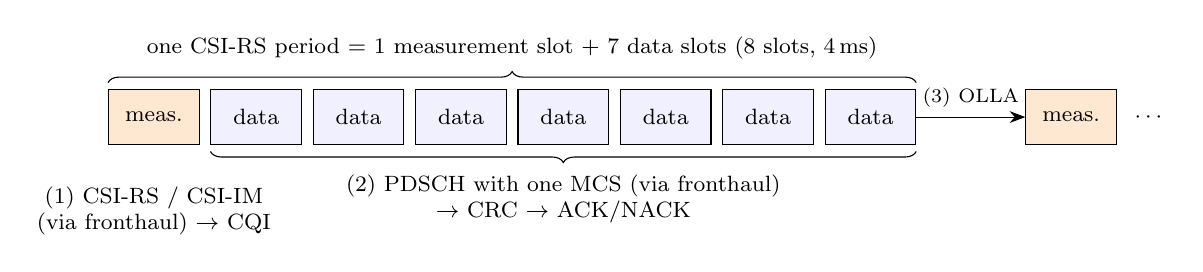
\begin{tikzpicture}[slot/.style={draw, minimum width=11.5mm, minimum height=7mm, font=\footnotesize, inner sep=1pt}]
  \node[slot, fill=orange!18] (s0) at (0,0) {meas.};
  \foreach \i in {1,...,7} \node[slot, fill=blue!6] (s\i) at (\i*1.3,0) {data};
  \node[slot, fill=orange!18] (n0) at (8*1.3+1.25,0) {meas.};
  \node[font=\footnotesize, right=1mm of n0] {$\cdots$};
  \draw[decorate, decoration={brace, amplitude=4pt}] ($(s0.north west)+(0,0.08)$) -- ($(s7.north east)+(0,0.08)$)
    node[midway, above=5pt, font=\footnotesize] {one CSI-RS period = 1 measurement slot + 7 data slots (8 slots, 4\,ms)};
  \draw[decorate, decoration={brace, amplitude=4pt, mirror}] ($(s1.south west)+(0,-0.08)$) -- ($(s7.south east)+(0,-0.08)$)
    node[midway, below=5pt, font=\footnotesize, align=center] {(2) PDSCH with one MCS (via fronthaul)\\$\to$ CRC $\to$ ACK/NACK};
  \node[font=\footnotesize, below=4mm of s0, align=center] {(1) CSI-RS / CSI-IM\\(via fronthaul) $\to$ CQI};
  \draw[->, >={Stealth[length=2mm]}] (s7.east) -- node[above, font=\scriptsize] {(3) OLLA} (n0.west);
\end{tikzpicture}
\caption{Closed-loop timing. (1) In the measurement slot the PDSCH is sent together with precoded CSI-RS and CSI-IM through the
fronthaul; the UE computes a CQI and reports it without errors or delay, and the MAC selects the MCS. (2) The following 7 data
slots use that MCS. (3) At the end of the period the OLLA offset is updated with all ACK/NACKs (equivalent to one period of HARQ
feedback delay).}
\label{fig:period}
\end{figure}

\paragraph{Measurement resources (TS 38.211 \S 7.4.1.5, TS 38.214 \S 5.2).} CSI-RS and CSI-IM are in symbol 12 of the
measurement slot. Each UE has one $\nu$-port NZP CSI-RS as channel measurement resource (CMR; for $\nu=2$ row 3 of Table
7.4.1.5.3-1, fd-CDM2, density 1); port $i$ is precoded with the BD weights of the UE's layer $i$. The co-scheduled UE's CMR doubles
as this UE's interference measurement resource (NZP-IMR). CSI-IM uses pattern 1 (4 subcarriers); powerControlOffset is 0\dB.
With 2 UEs $\times$ 2 layers, subcarriers 0--3 of each PRB are CMR and 4--7 CSI-IM. The PDSCH of the measurement slot is punctured
on these REs (the specification rate-matches around them), so that the content of the compressed fronthaul blocks is realistic;
that slot is not decoded. In Cat A the CSI-RS is precoded in the O-DU together with the PDSCH; in Cat B it sits in the
corresponding layer stream and is precoded in the O-RU with the (compressed) weights.

\paragraph{CQI computation at the UE (reportQuantity = cri-RI-CQI, no PMI).}
\begin{enumerate}
  \item compensate the timing with the phase slope estimated from the PDSCH DMRS;
  \item in each PRB, LS on the 2 CMR REs + CDM2 despreading gives the $N_r \times \nu$ effective channel;
  \item take the mean power on the CSI-IM as the noise variance (\textbf{zeros stay zero after compression, so no compression
        distortion is measured here});
  \item take the interference covariance from the co-scheduled UE's NZP-IMR, averaged over the PRG, minus the estimation noise
        $\nu\sigma^2/2$ (without this correction the interference in the BD nulls is overestimated to the level of the noise,
        and the MU SINR is underestimated by about 3\dB);
  \item compute the LMMSE SINR $\gamma_i$ per PRB and layer and combine them with EESM,
        \begin{equation}
          \gamma_{\mathrm{eff}} = -\beta \ln\!\Big( \frac{1}{N} \sum_{i=1}^{N} e^{-\gamma_i/\beta} \Big),
        \end{equation}
        then report the highest CQI with AWGN TBLER $\le 0.1$ (TS 38.214 \S 5.2.2.1). The TBS uses the CSI reference resource
        (\S 5.2.2.5.1: symbols 2--13 minus DMRS, i.e.\ 10 data symbols; the actual PDSCH has 12). The rank is fixed; no RI is
        reported.
\end{enumerate}
For comparison, a ``genie CQI'' is always computed from the true effective channel $\mathbf H_k \mathbf W$ with per-RE LMMSE SINR,
bypassing the fronthaul. With an ideal fronthaul, the CSI-RS CQI is within 1 of the genie CQI (unit test).

\paragraph{MAC link adaptation (\code{link_adaptation.py}).} 3GPP does not specify the algorithm. Here the CQI is mapped to its
threshold SINR $\gamma_{\mathrm{th}}(\mathrm{CQI})$ (a conservative lower bound), the OLLA offset $\Delta$ is added, and the
highest MCS whose threshold (computed for the actual number of allocated REs) does not exceed the result is chosen:
\begin{equation}
  \mathrm{MCS} = \max\{ m : \gamma_{\mathrm{th}}^{\mathrm{MCS}}(m) \le \gamma_{\mathrm{th}}(\mathrm{CQI}) + \Delta \}.
\end{equation}
OLLA updates $\Delta \leftarrow \Delta + \delta\, p/(1-p)$ on every ACK and $\Delta \leftarrow \Delta - \delta$ on every NACK, so
that the first-transmission BLER converges to the target $p = 0.1$; $\delta = 0.5$\dB, $\Delta \in [-10, 10]$\dB, and no further
increase once the highest MCS is reached. $\Delta = 0$ is plain CQI table lookup (used in F1). There are no HARQ retransmissions.
The AWGN thresholds come from Sionna SYS's PDSCH BLER tables (per code-block length, combined into a TBLER through TB
segmentation); the EESM $\beta$ values are Sionna's calibrated ones.

\paragraph{Usable MCS.} Sionna's LDPC encoder does not support repetition, so MCSs with very low code rates cannot be built.
Trying to build the coding chain for each MCS shows that MCS table 2 indices 3--27 are usable. UEs below the MCS 3 threshold
(about 0.6\dB) can only run at high BLER.

\subsection{Metrics}

\begin{description}[leftmargin=1.2em, style=nextline, itemsep=1pt]
  \item[SNR (open loop)] total transmit power per RE is 1 and the average gain per TX--RX antenna pair is 1, so
        $\mathrm{SNR} = 1/N_0$.
  \item[Required SNR and loss] the SNR at which the BLER averaged over both UEs first falls below 0.1 (linear interpolation of
        $\log_{10}\mathrm{BLER}$); the loss is the difference to the ideal fronthaul.
  \item[U-plane SQNR] signal-to-quantization-noise ratio of the fronthaul IQ after fixed point and compression.
  \item[TX EVM] error of the frequency-domain signal at the O-RU antennas relative to an ideal fronthaul (no quantization,
        no compression); it reflects fronthaul distortion only.
  \item[RX EVM] error of the equalized data symbols at the UE relative to the transmitted ones (noise, interference, channel
        estimation error and compression distortion).
  \item[Wideband SNR (closed loop)] $P_{\mathrm{RE}} \cdot \overline{|h|^2} / N_0$ per receive antenna with equal power on all
        transmit antennas, without beamforming or receive-combining gain.
  \item[Throughput (closed loop)] bits of TBs decoded correctly at the first transmission in the data slots after the
        warm-up, divided by the duration of the data slots (no HARQ).
  \item[Measured data-slot SINR] power of the equalized transmitted symbols over the error power on the data slots: the SINR
        the PDSCH actually experiences.
  \item[CQI overestimate] effective SINR measured by the CSI minus the measured data-slot SINR; this report gives its increase
        relative to the ideal fronthaul.
  \item[$\Delta$CQI] in E3, CSI-RS CQI minus genie CQI; in F1, CQI minus the CQI with ideal fronthaul.
  \item[INR (NZP-IMR)] interference power measured by the UE on the co-scheduled UE's CSI-RS over the CSI-IM noise.
  \item[OLLA offset] mean offset after the warm-up; a negative value means the MAC has to lower the CQI-derived SINR by that
        many dB to reach the BLER target.
  \item[Fronthaul load] U-plane + C-plane bit rate of one O-RU link including eCPRI and Ethernet overhead, also scaled to
        100\,MHz (273 PRBs).
\end{description}

\subsection{Main simplifications}

\begin{itemize}
  \item PDSCH: Sionna 2.2 only has PUSCH. \code{PDSCHConfig} inherits from \code{PUSCHConfig} and only changes the TB channel
        type (MCS table, scrambling initialization); with CP-OFDM the DMRS and TBS calculations are identical. The $\lambda$
        term in the DMRS sequence initialization is 0 (equivalent to Rel-18 for Type 1 DMRS without dmrs-Downlink-r16).
  \item Simulation in the frequency domain by default (time-domain mode with a 1024-point IFFT at 30.72\,Msps gives identical
        results, verified by unit tests); the time-domain quantization of option 8 is modelled separately. In time-domain mode
        the CIR is drawn once per OFDM symbol (Doppler within a symbol is ignored).
  \item Precoding from ideal CSI (TDD reciprocity) at the PRG centre; CSI reports without errors or delay; fixed rank, no RI
        adaptation; no HARQ.
  \item Static UEs; full buffer, all UEs on all PRBs; one MCS per batch (CSI-RS period).
  \item For Cat B modulation compression, the C-plane bytes of SE 5 / SE 6 and of the DMRS section are estimated from the
        formats; the second SE 5 mask set in the measurement slot is ignored.
\end{itemize}

% =====================================================================
\section{E1: open-loop Cat A / Cat B $\times$ compression width $\times$ SNR}
% =====================================================================

\subsection{Setup}

\begin{table}[H]
\centering
\caption{Setup of E1 / E1$'$ (\code{compare_cat_a_b.py})}
\label{tab:e1setup}
\footnotesize
\begin{tabularx}{\textwidth}{@{}P{3.0cm} Y@{}}
\toprule
Item & Setting \\
\midrule
Carrier & 30\,kHz SCS, 51 PRBs (20\,MHz), 3.5\,GHz; frequency-domain simulation \\
Nodes & 1 O-RU with 8 TX chains ($1\times4$ dual-polarized); 2 UEs with 4 antennas each ($1\times2$ dual-polarized); 2 layers per UE,
        4 in total \\
PDSCH & MCS table 2 index 20 (256QAM, $R = 682.5/1024$); TBS 77896 bit per UE and slot \\
Precoding / receiver & BD, PRG 2 PRBs; PRG-aware DMRS LS estimation + LMMSE at the UE \\
Channel & CDL-C, 100\,ns delay spread, static UEs \\
Fronthaul & U-plane: ideal, BFP 9/7/6/5/4 bit (E1); BFP / block scaling / $\mu$-law at 6 and 5 bit plus block scaling at 4 bit
            (E1$'$). \textbf{Cat B weights fixed at BFP 9 bit} (unquantized with the ideal fronthaul) \\
SNR and samples & 14--30\dB in 2\dB steps; 16 slots per batch, at most 20 batches per SNR point, stop after 100 block errors;
                  seed 42 \\
Execution & Cat A and Cat B on two GPUs, both mapped to \code{cuda:0} with \code{CUDA_VISIBLE_DEVICES} so that bits, channels
            and noise are identical on both sides (paired comparison); merged with \code{--merge} \\
\bottomrule
\end{tabularx}
\end{table}

\subsection{BFP width sweep}

\begin{table}[H]
\centering
\caption{E1: fronthaul load and link performance of Cat A / Cat B for different BFP widths (one O-RU, including eCPRI /
Ethernet overhead)}
\label{tab:e1}
\footnotesize
\begin{tabular}{@{}l l r r r r r r r r@{}}
\toprule
 & & \multicolumn{2}{c}{Fronthaul (Gbit/s)} & SQNR & TX EVM & Req.\ SNR & Loss & \multicolumn{2}{c}{at 30\,dB} \\
\cmidrule(lr){3-4}\cmidrule(lr){9-10}
Cat & U-plane & 20\,MHz & 100\,MHz & (dB) & (\%) & (dB) & (dB) & BLER & RX EVM (\%) \\
\midrule
A & ideal   & 4.61 & 24.57 & $\infty$ & 0     & 23.10 & 0.00 & 0.0016 & 6.27 \\
B & ideal   & 2.36 & 12.59 & $\infty$ & 0     & 23.10 & 0.00 & 0.0016 & 6.27 \\
\midrule
A & BFP 9  & 2.67 & 14.35 & 49.2 & 0.345 & 23.10 & 0.00 & 0.0016 & 6.29 \\
B & BFP 9  & 1.37 &  7.36 & 50.7 & 0.438 & 23.12 & 0.02 & 0.0016 & 6.26 \\
\midrule
A & BFP 7  & 2.13 & 11.31 & 37.2 & 1.381 & 23.16 & 0.06 & 0.0031 & 6.65 \\
B & BFP 7  & 1.10 &  5.84 & 38.5 & 1.237 & 23.12 & 0.02 & 0.0016 & 6.39 \\
\midrule
A & BFP 6  & 1.85 &  9.73 & 31.2 & 2.763 & 23.69 & 0.59 & 0.027  & 7.67 \\
B & BFP 6  & 0.96 &  5.05 & 32.2 & 2.483 & 23.35 & 0.25 & 0.0016 & 7.08 \\
\midrule
A & BFP 5  & 1.58 &  8.16 & 25.1 & 5.530 & ---   & ---  & 0.211  & 10.93 \\
B & BFP 5  & 0.82 &  4.27 & 27.1 & 4.428 & 23.97 & 0.87 & 0.0094 & 7.97 \\
\midrule
A & BFP 4  & 1.30 &  6.69 & 19.1 & 11.07 & ---   & ---  & 1.0    & 19.68 \\
B & BFP 4  & 0.69 &  3.53 & 20.5 & 9.477 & ---   & ---  & 1.0    & 12.45 \\
\bottomrule
\end{tabular}

\smallskip
\parbox{\textwidth}{\footnotesize ``---'': the BLER never fell below 0.1 up to 30\dB. The Cat B load includes the C-plane
weights: about 0.19\Gbps with BFP 9 weights and 0.31\Gbps with ideal (16-bit) weights at 100\,MHz.}
\end{table}

\begin{figure}[H]
\centering
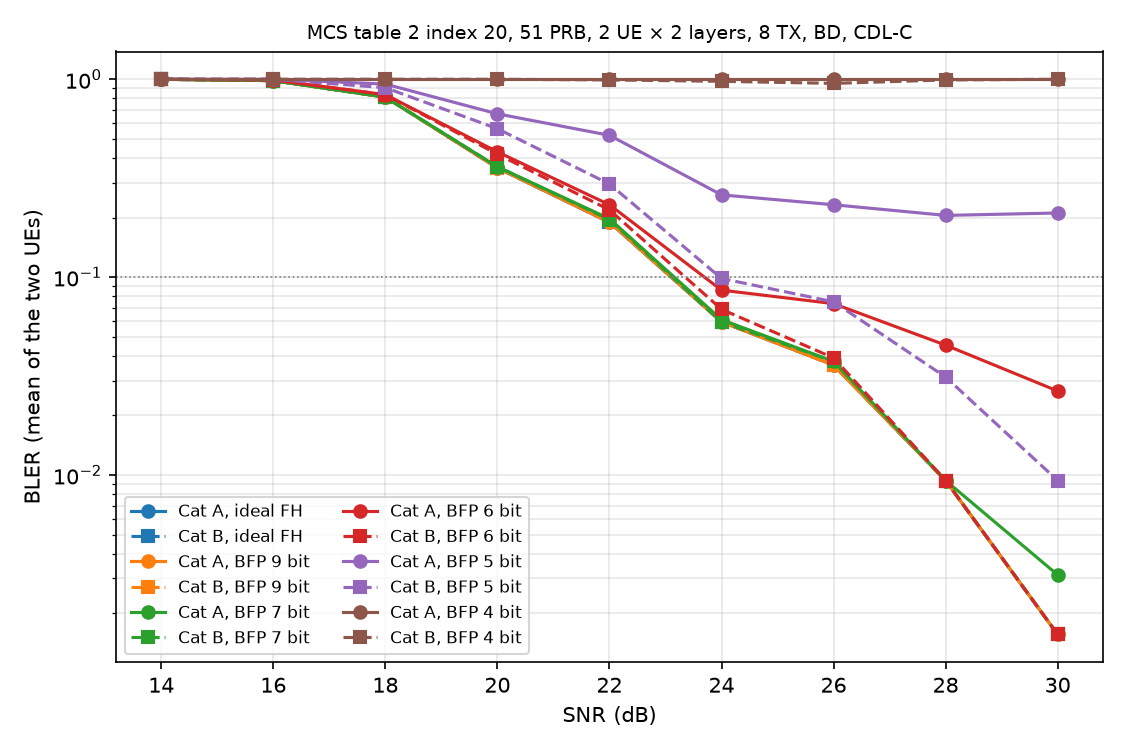
\includegraphics[width=0.78\textwidth]{figures/e1_cat_ab_bler.png}
\caption{E1: BLER (mean of both UEs) versus SNR. Solid lines Cat A, dashed lines Cat B, colours the BFP width; the dotted grey
line marks BLER $=0.1$. Ideal, 9-bit and 7-bit curves almost coincide; Cat A at 5 bit has an error floor near 0.21; neither
category works at 4 bit.}
\label{fig:e1bler}
\end{figure}

\begin{figure}[H]
\centering
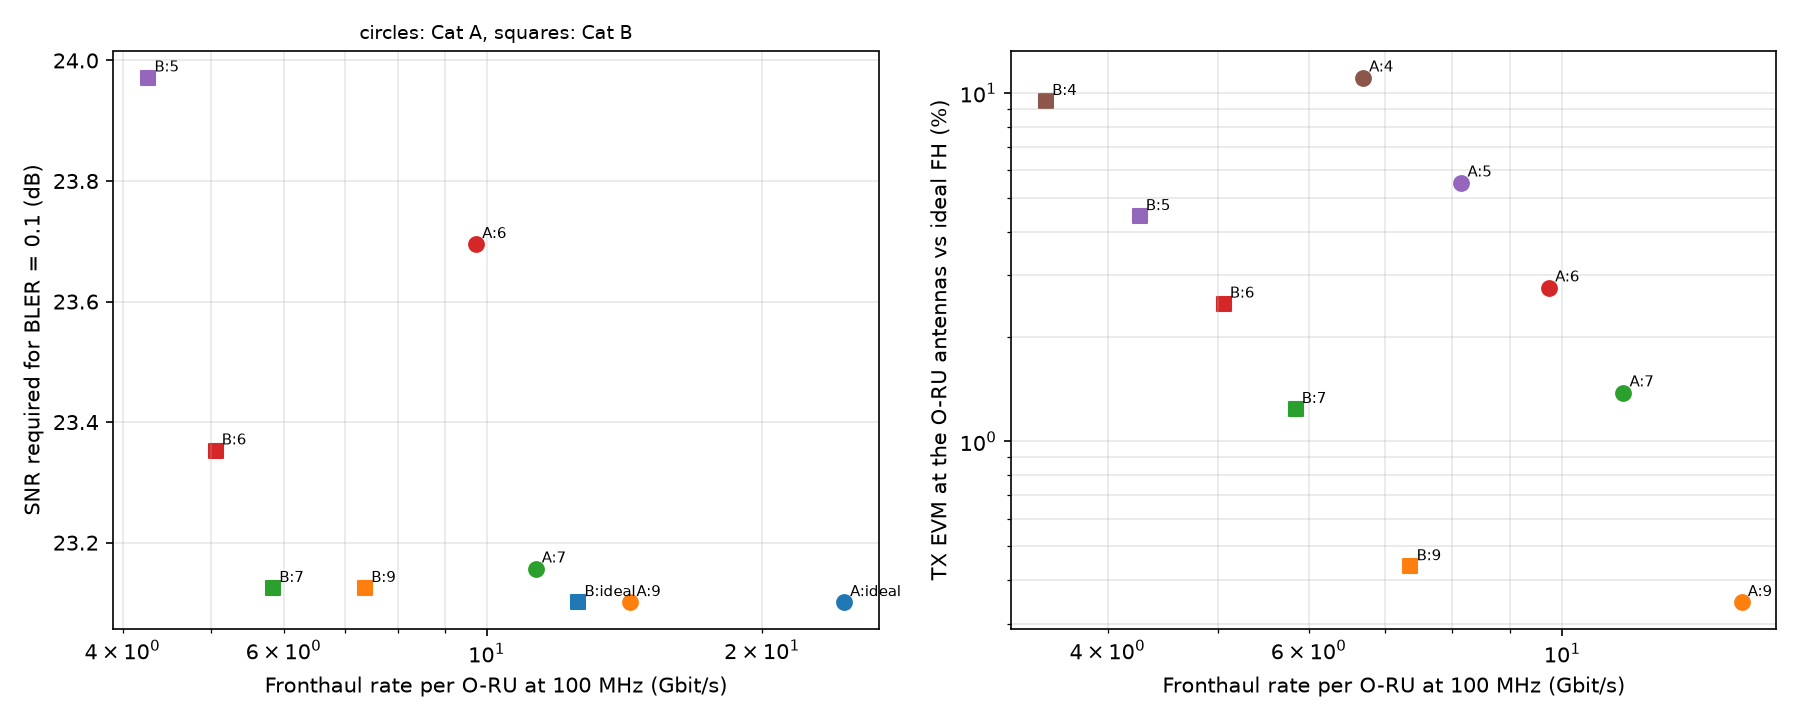
\includegraphics[width=\textwidth]{figures/e1_cat_ab_tradeoff.png}
\caption{E1: fronthaul rate of one O-RU (100\,MHz) against the required SNR (left) and the TX EVM (right). Circles Cat A,
squares Cat B; labels read ``category:width''.}
\label{fig:e1tradeoff}
\end{figure}

\subsection{Compression methods (E1$'$)}

\begin{table}[H]
\centering
\caption{E1$'$: the three block methods at equal width. Equal width means equal load: at 100\,MHz, 6 bit is 9.73 (Cat A) /
5.05\Gbps (Cat B), 5 bit 8.16 / 4.27\Gbps, 4 bit 6.69 / 3.53\Gbps.}
\label{tab:e1m}
\footnotesize
\begin{tabular}{@{}l l r r r r r@{}}
\toprule
Cat & U-plane & SQNR (dB) & TX EVM (\%) & Req.\ SNR (dB) & Loss (dB) & BLER at 30\,dB \\
\midrule
A & BFP 6             & 31.2 & 2.763 & 23.69 & 0.59 & 0.025 \\
A & block scaling 6   & 33.7 & 2.056 & 23.40 & 0.30 & 0.011 \\
A & $\mu$-law 6       & 31.1 & 2.777 & 23.76 & 0.66 & 0.030 \\
A & BFP 5             & 25.1 & 5.530 & ---   & ---  & 0.211 \\
A & block scaling 5   & 27.5 & 4.208 & 29.06 & 5.96 & 0.089 \\
A & $\mu$-law 5       & 25.0 & 5.615 & ---   & ---  & 0.234 \\
A & block scaling 4   & 21.3 & 8.591 & ---   & ---  & 0.961 \\
\midrule
B & BFP 6             & 32.2 & 2.483 & 23.35 & 0.25 & 0.0016 \\
B & block scaling 6   & 37.8 & 1.333 & 23.18 & 0.08 & 0.0016 \\
B & $\mu$-law 6       & 32.3 & 2.461 & 23.56 & 0.46 & 0.0016 \\
B & BFP 5             & 27.1 & 4.428 & 23.97 & 0.87 & 0.0094 \\
B & block scaling 5   & 29.1 & 3.542 & 23.58 & 0.48 & 0.0016 \\
B & $\mu$-law 5       & 25.1 & 5.590 & 23.42 & 0.32 & 0.0031 \\
B & block scaling 4   & 21.7 & 8.253 & ---   & ---  & 1.0 \\
\bottomrule
\end{tabular}
\end{table}

\subsection{Analysis}

\begin{enumerate}
  \item \textbf{Simulator consistency.} With an ideal fronthaul, Cat A and Cat B both need 23.10\dB, and their BLER and RX EVM
        at 30\dB are identical. The two signal paths (precoding in the O-DU and in the O-RU) are thus implemented consistently,
        in line with the unit test that checks bit-identical air-interface signals.
  \item \textbf{Fronthaul load.} Here Cat A carries 8 antenna streams and Cat B 4 layer streams, so at equal width the Cat B
        U-plane is exactly half of Cat A's; Cat B pays another 0.19\Gbps of C-plane for BFP 9 weights. BFP at $w$ bit costs
        $24w+8$ bit per PRB; relative to 16-bit uncompressed (384 bit per PRB) that is 58\% at 9 bit, 46\% at 7 bit and 33\% at
        5 bit, which matches the loads in the table.
  \item \textbf{SQNR is about 6\dB per bit} (BFP 9/7/6/5/4: 49.2 / 37.2 / 31.2 / 25.1 / 19.1\dB), as expected for uniform
        quantization. At equal width Cat B has 1--2\dB more SQNR than Cat A. A plausible reason is that layer-domain signals are
        bounded QAM points with a lower peak-to-average ratio within a block than the near-Gaussian sum of several precoded
        layers on an antenna, which suits a shared block exponent better.
  \item \textbf{Bit-width thresholds.} 9 and 7 bit are practically lossless ($\le 0.06$\dB) and cut the load to 58\% and 46\% of
        uncompressed. 6 bit starts to cost (Cat A 0.59\dB, Cat B 0.25\dB). \textbf{5 bit is the breaking point}: Cat A shows an
        error floor near 0.21 and Cat B loses 0.87\dB. At 4 bit (SQNR about 20\dB) neither supports 256QAM. The AWGN threshold of
        256QAM at rate 0.67 is about 19\dB (CQI 12, 256QAM at rate 0.69, needs 19.2\dB), and with BD and channel estimation the
        link needs 23.1\dB SNR; a transmit-side SQNR of 20\dB is therefore already below the operating point.
  \item \textbf{Why Cat A is more sensitive with MU.} In Cat A the compression noise is in the antenna domain, spatially white
        and not precoded, so BD cannot null it towards the co-scheduled UE. A UE receives the distortion of its own signal and of
        the other UE's signal. In Cat B the noise is in the layer domain, is sent with this UE's weights and is nulled at the
        co-scheduled UE by BD. At 5 bit and 30\dB, the RX EVM is therefore 10.9\% for Cat A and 8.0\% for Cat B. (With a single
        user the ranking reverses; see E3.)
  \item \textbf{Compression methods.} The block-scaling factor is finer than a power-of-two exponent, giving 2.0--5.6\dB more
        SQNR than BFP at equal width and the smallest loss (Cat A at 6 bit: 0.30 vs 0.59\dB). $\mu$-law has about the same SQNR as
        BFP. SQNR alone does not predict the BLER loss, though: for Cat B at 5 bit, $\mu$-law has the lowest SQNR (25.1\dB) but
        loses only 0.32\dB, less than BFP (0.87\dB). The Cat B U-plane carries the QAM points themselves, so the quantization
        error is deterministic (it depends on where the constellation points lie relative to the quantizer grid) rather than
        noise-like, and a single SQNR number cannot describe it (the F1 constellations show this clearly).
\end{enumerate}

% =====================================================================
\section{E2: ray-traced closed-loop baseline (SU / MU)}
% =====================================================================

\subsection{Setup}

30 random drops in the munich scene; for each drop 16 CSI-RS periods with 8 data slots per period sharing one MCS; the first
4 periods (OLLA convergence) are excluded. Seeds start at 1 and increase by one per drop. Fronthaul Cat A with BFP 9-bit
U-plane; MCS and CQI table 2; OLLA step 0.5\dB, BLER target 0.1. SU is 1 UE $\times$ 2 layers; MU is 2 UEs $\times$ 2 layers
with BD.

\textbf{Note:} E2 ran before the CSI-RS implementation (5 October 2026 19:10, before commit \code{e4fedff} that added the
CSI-RS). At that time the UE computed the CQI directly from the true effective channel on the CSI reference resource, which is
equivalent to today's genie CQI and bypasses the fronthaul; there was no separate measurement slot. E2 is therefore a closed-loop
baseline with ideal CSI measurement.

\subsection{Results}

\begin{table}[H]
\centering
\caption{E2: ray-traced closed-loop baseline (30 drops; one sample per UE)}
\label{tab:e2}
\footnotesize
\begin{tabular}{@{}l r r@{}}
\toprule
 & SU (1 UE $\times$ 2 layers) & MU (2 UEs $\times$ 2 layers, BD) \\
\midrule
Wideband SNR, median / range (dB)                & 38.2 / $-16.5$ to 53.4 & 39.8 / $-16.5$ to 54.5 \\
Effective SINR of the CQI, median (dB)           & 41.4 & 29.9 \\
Mean CQI; share of UEs with CQI $=15$            & 13.3; 77\% & 13.0; 67\% \\
Mean MCS; share of UEs always at MCS 27          & 23.0; 73\% & 22.4; 53\% \\
Mean first-transmission BLER                     & 0.056 & 0.088 \\
Mean final OLLA offset (dB)                      & $-0.58$ & $-0.73$ \\
UE throughput: mean / median / 5th pct.\ (Mbit/s) & 197.5 / 237.8 / 38.5 & 172.3 / 217.1 / 25.2 \\
Sum throughput per drop, mean (Mbit/s)           & 197.5 & 344.6 \\
\bottomrule
\end{tabular}
\end{table}

\begin{figure}[H]
\centering
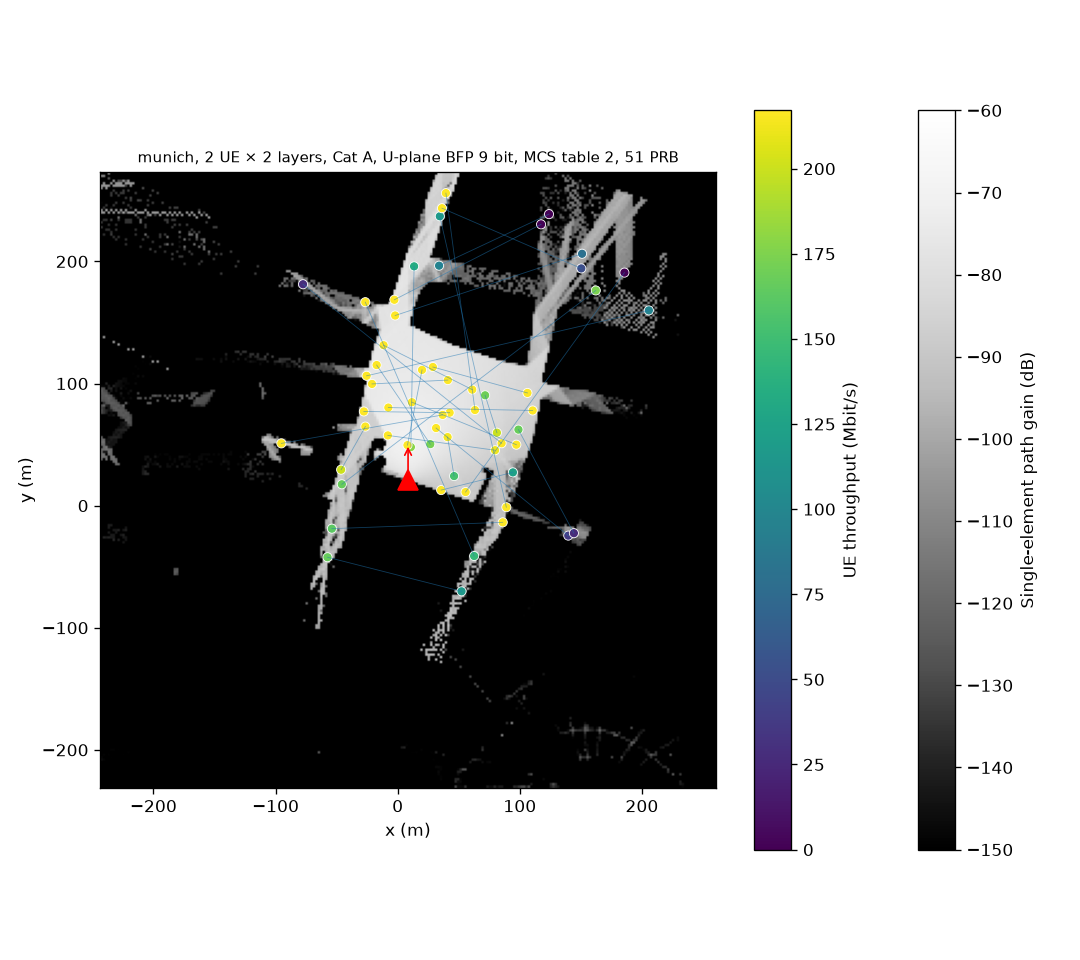
\includegraphics[width=0.72\textwidth]{figures/e2_rt_mu_map.png}
\caption{E2 (MU): single-element path-gain coverage map of the munich scene (grey scale), O-RU position and boresight (red
triangle and arrow), and the UE positions of all drops (colour = throughput; thin lines connect the two UEs of a drop). The
square and streets north of the O-RU form the main coverage area; distant UEs that are shadowed by buildings and reached only by
diffraction have the lowest throughput.}
\label{fig:e2map}
\end{figure}

\subsection{Analysis}

\begin{enumerate}
  \item \textbf{High SNR; most UEs sit at the top MCS.} With one O-RU at 35\,dBm over 20\,MHz, the median wideband SNR is close to
        40\dB. In SU, 73\% of the UEs stay at MCS 27 all the time, and the median throughput equals the peak (237.8\,Mbit/s). The
        throughput spread comes from a few shadowed UEs.
  \item \textbf{MU is limited by residual multi-user interference, not by noise.} The SNR distributions are similar, but the
        median effective SINR in MU is about 11\dB lower than in SU (29.9 vs 41.4\dB): BD nulls only at the PRG centre, and the
        large delay spread of the ray-traced channel leaves residual interference within each PRG.
  \item \textbf{The lower MU peak is DMRS overhead.} In MU neither CDM group carries data (7344 data REs per layer and slot); in SU
        only one CDM group is left empty, so there are more data REs. At MCS 27 a UE therefore gets 237.8\,Mbit/s in SU and
        217.1\,Mbit/s in MU. Per drop, MU delivers 1.74 times the SU throughput.
  \item \textbf{OLLA behaviour.} For static UEs the BLER-versus-MCS relation is close to a step, so OLLA toggles around the
        step. UEs at the top MCS cannot go higher, so the mean first-transmission BLER (0.056 / 0.088) stays below the 0.1 target.
\end{enumerate}

% =====================================================================
\section{E3: visibility of compression distortion in the closed loop}
% =====================================================================

\subsection{Setup}

E3 adds CSI-RS measurement to the E2 closed loop (Section~\ref{sec:closedloop}): one CSI-RS period is 1 measurement slot +
7 data slots, the CQI comes from CSI-RS / CSI-IM sent through the fronthaul, and OLLA is on. U-plane: ideal, BFP 9 / 7 / 5 bit.
\textbf{Cat B weights use the same method and width as the U-plane} (unlike E1). 30 drops, 16 periods, first 4 excluded, seed 1.

The drops are generated first with \code{--save-drops} and stored in \code{drops_su.json} / \code{drops_mu.json}; the two GPUs read
the same drop file and run Cat A and Cat B respectively. All compression settings are run in turn on the same drop, each starting
from the same seed, so channel, bits and noise are identical across settings (paired comparison). The shared drop file is needed
because the coverage map is a Monte Carlo result: when each process drops its own UEs, a few drops near the acceptance threshold
can differ.

\subsection{Results}

\begin{table}[H]
\centering
\caption{E3: closed-loop performance per compression setting (throughput in Mbit/s; fronthaul for one O-RU at 100\,MHz)}
\label{tab:e3}
\footnotesize
\setlength{\tabcolsep}{4.5pt}
\begin{tabular}{@{}l l l r r r r r r r r@{}}
\toprule
Case & Cat & U-plane & FH (Gbit/s) & Mean tput & 5\% tput & BLER & OLLA (dB) & $\Delta$CQI & INR (dB) & MCS \\
\midrule
\multirow{8}{*}{SU} & A & ideal  & 24.57 & 196.0 & 11.4 & 0.088 & $-0.92$ & $+0.14$ & --- & 22.9 \\
                    & A & BFP 9  & 14.35 & 195.9 & 11.4 & 0.088 & $-0.92$ & $+0.14$ & --- & 22.9 \\
                    & A & BFP 7  & 11.31 & 195.9 & 11.4 & 0.088 & $-0.94$ & $+0.14$ & --- & 22.9 \\
                    & A & BFP 5  &  8.16 & 189.2 & 11.4 & 0.099 & $-1.32$ & $+0.14$ & --- & 22.4 \\
\cmidrule(l){2-11}
                    & B & ideal  &  6.30 & 196.0 & 11.4 & 0.088 & $-0.92$ & $+0.14$ & --- & 22.9 \\
                    & B & BFP 9  &  3.68 & 195.7 & 11.4 & 0.088 & $-0.93$ & $+0.14$ & --- & 22.9 \\
                    & B & BFP 7  &  2.90 & 195.7 & 12.0 & 0.088 & $-0.98$ & $+0.15$ & --- & 22.9 \\
                    & B & BFP 5  &  2.10 & 120.3 & 11.4 & 0.189 & $-6.52$ & $+0.13$ & --- & 16.8 \\
\midrule
\multirow{8}{*}{MU} & A & ideal  & 24.57 & 173.3 & 25.2 & 0.087 & $-0.48$ & $+0.00$ & 19.5 & 22.5 \\
                    & A & BFP 9  & 14.35 & 172.1 & 25.2 & 0.090 & $-0.55$ & $+0.00$ & 19.5 & 22.4 \\
                    & A & BFP 7  & 11.31 & 166.4 & 25.2 & 0.093 & $-1.07$ & $-0.05$ & 19.8 & 21.8 \\
                    & A & BFP 5  &  8.16 & 112.3 &  4.5 & 0.184 & $-5.13$ & $-0.46$ & 23.0 & 16.6 \\
\cmidrule(l){2-11}
                    & B & ideal  & 12.59 & 173.3 & 25.2 & 0.087 & $-0.47$ & $+0.00$ & 19.5 & 22.5 \\
                    & B & BFP 9  &  7.36 & 172.9 & 25.2 & 0.088 & $-0.49$ & $+0.00$ & 19.5 & 22.5 \\
                    & B & BFP 7  &  5.81 & 171.1 & 25.2 & 0.092 & $-0.62$ & $+0.01$ & 19.8 & 22.4 \\
                    & B & BFP 5  &  4.20 & 153.4 & 21.9 & 0.115 & $-1.64$ & $-0.25$ & 22.0 & 20.7 \\
\bottomrule
\end{tabular}

\smallskip
\parbox{\textwidth}{\footnotesize $\Delta$CQI $=$ CSI-RS CQI $-$ genie CQI. INR is the interference-to-noise ratio measured on the
NZP-IMR; SU has no co-scheduled UE and hence no INR. OLLA is the mean offset after the warm-up.}
\end{table}

To separate what the CSI sees from what the PDSCH experiences, Table~\ref{tab:e3sinr} gives two SINR changes relative to the
ideal fronthaul (dB, averaged over all UEs). The drop of the measured data-slot SINR is the true cost of the distortion; the drop
of the CSI effective SINR is the part the CQI can see; their difference is the increase of the CQI overestimate, which only OLLA
can absorb.

\begin{table}[H]
\centering
\caption{E3: SINR changes relative to the ideal fronthaul (dB, mean over all UEs)}
\label{tab:e3sinr}
\footnotesize
\begin{tabular}{@{}l l r r r r r r@{}}
\toprule
 & & \multicolumn{3}{c}{SU} & \multicolumn{3}{c}{MU} \\
\cmidrule(lr){3-5}\cmidrule(lr){6-8}
Cat & U-plane & data SINR & CSI SINR & CQI overest. & data SINR & CSI SINR & CQI overest. \\
\midrule
A & BFP 9 & $-0.49$  & $0.00$  & $+0.49$  & $-0.41$  & $-0.10$ & $+0.32$ \\
A & BFP 7 & $-3.32$  & $0.00$  & $+3.32$  & $-3.10$  & $-1.02$ & $+2.08$ \\
A & BFP 5 & $-10.09$ & $-0.01$ & $+10.08$ & $-10.09$ & $-4.43$ & $+5.66$ \\
\midrule
B & BFP 9 & $-0.77$  & $-0.01$ & $+0.77$  & $-0.37$  & $-0.05$ & $+0.32$ \\
B & BFP 7 & $-6.52$  & $+0.08$ & $+6.60$  & $-2.13$  & $-0.66$ & $+1.48$ \\
B & BFP 5 & $-12.77$ & $+0.28$ & $+13.05$ & $-8.12$  & $-3.32$ & $+4.80$ \\
\bottomrule
\end{tabular}
\end{table}

\begin{figure}[H]
\centering
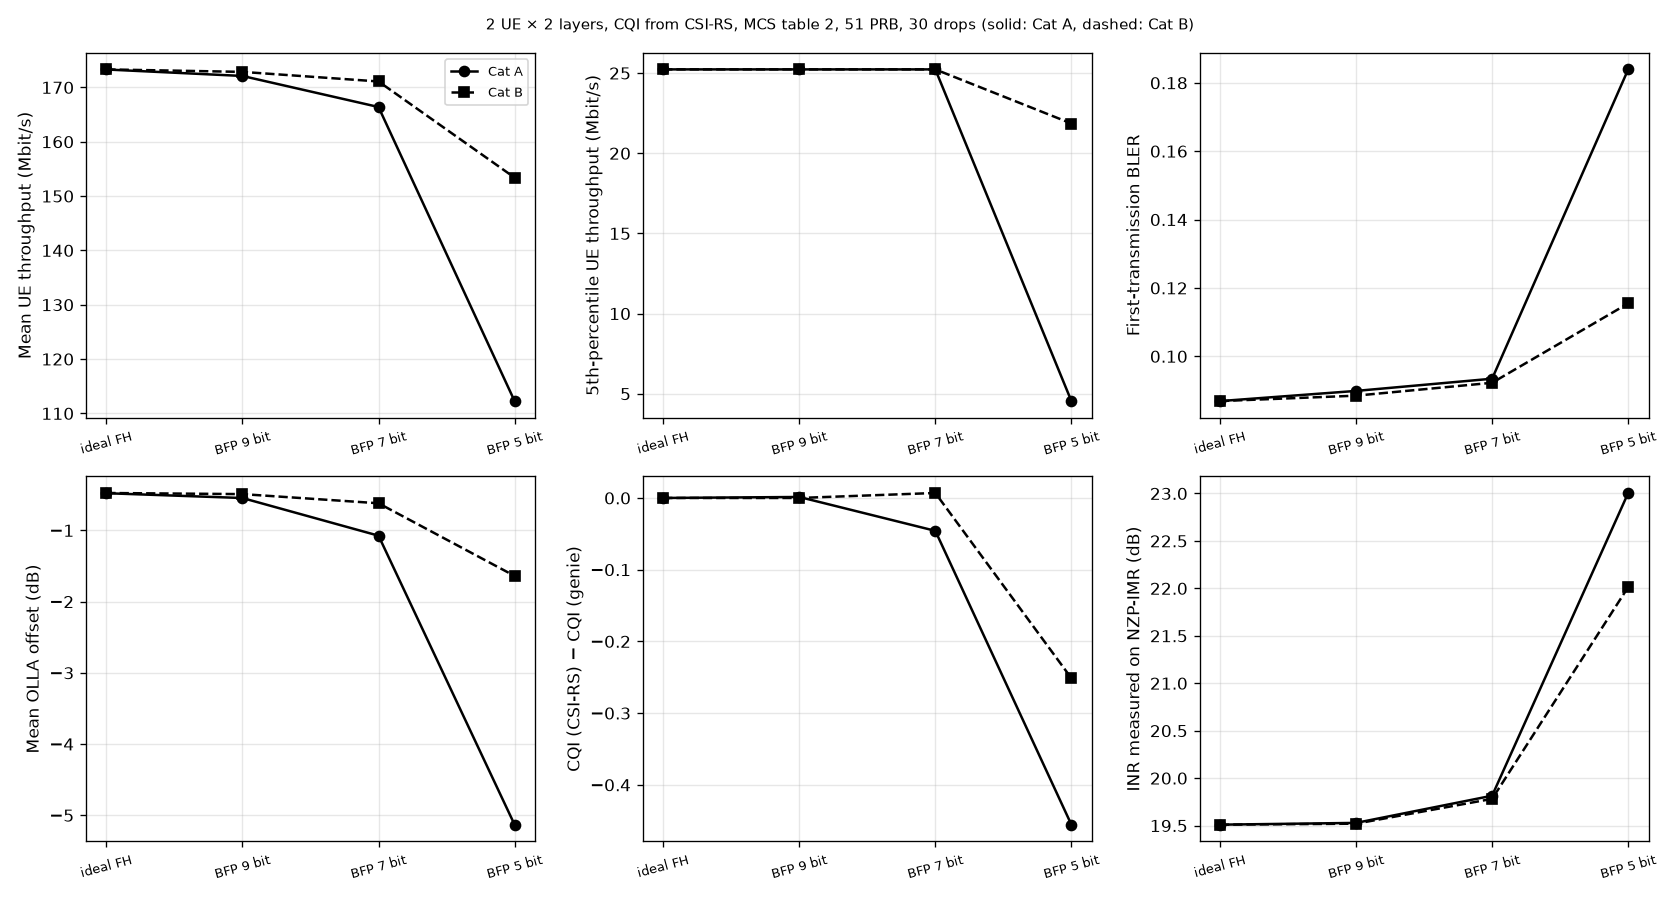
\includegraphics[width=\textwidth]{figures/e3_csi_mu_summary.png}
\caption{E3 (MU, 2 UEs $\times$ 2 layers): mean and 5th-percentile throughput, first-transmission BLER, mean OLLA offset, CQI
relative to the genie CQI, and INR measured on the NZP-IMR versus the compression setting. Solid Cat A, dashed Cat B.}
\label{fig:e3}
\end{figure}

\subsection{Analysis}

\begin{enumerate}
  \item \textbf{The CSI-IM sees nothing, and with SU the CSI-RS hardly sees anything.} In SU the CSI effective SINR barely moves
        ($|\Delta| \le 0.3$\dB) and $\Delta$CQI stays at about $+0.14$, while the measured data-slot SINR drops by 0.5--12.8\dB.
        SU has no co-scheduled UE and therefore no NZP-IMR; the CSI-IM is zero after compression; self-distortion only appears as
        CMR channel-estimation error, which the UE does not count as interference. With SU the compression distortion is thus
        invisible to the CQI and must be absorbed entirely by OLLA.
  \item \textbf{With MU the NZP-IMR sees 30--45\%.} At 5 bit, the Cat A data SINR drops by 10.1\dB of which the CSI sees
        4.4\dB (44\%); for Cat B it is 8.1 and 3.3\dB (41\%). At 7 bit the shares are 33\% (Cat A) and 31\% (Cat B). The visible part comes from the co-scheduled UE's CSI-RS distortion
        leaking into this UE (Cat A) and from weight compression degrading the BD nulls (Cat B); both are measured on the NZP-IMR
        (INR rises from 19.5 to 22--23\dB). The invisible part (self-distortion) can only be absorbed by OLLA, which is why the
        OLLA offset deepens as the width shrinks (Cat A at 5 bit: $-5.1$\dB).
  \item \textbf{A large SINR drop does not necessarily cost throughput.} In SU, Cat B at 7 bit lowers the data SINR by 6.5\dB on
        average while the throughput is unchanged (195.7 vs 196.0): most UEs are far above the MCS 27 threshold and the distortion
        only eats their margin. The dB averages are dominated by these high-SNR, distortion-limited UEs.
  \item \textbf{Cat A and Cat B swap places between SU and MU.} With SU, Cat B is more sensitive (throughput 120.3 at 5 bit vs
        189.2 for Cat A). The Cat B layer-domain noise is beamformed together with the signal and gets the same array gain, so
        the transmit-side SQNR reaches the UE almost unchanged; the white antenna-domain noise of Cat A is spread over an
        8-dimensional space, of which only a part falls into the UE's signal subspace, while the signal itself enjoys the
        beamforming gain. The Cat B weights are also compressed to 5 bit in this experiment. With MU, Cat A is more sensitive
        (112.3 vs 153.4 at 5 bit), for the reason given in E1, item 5: antenna-domain noise cannot be nulled by BD and leaks to
        the co-scheduled UE.
  \item \textbf{7 bit is a safe width in the closed loop.} With BFP 7, MU throughput drops by 4\% (Cat A) and 1.3\% (Cat B), SU
        by less than 0.2\% for both; at 9 bit all metrics are practically identical to the ideal fronthaul.
\end{enumerate}

% =====================================================================
\section{F1: fronthaul load of four functional splits in cell-free MIMO}
% =====================================================================

\subsection{Purpose and setup}

F1 compares the fronthaul load of option 7-1, 7.2x Cat A, 7.2x Cat B and option 8 in the same cell-free downlink, together with
the throughput cost of each split's compression schemes in a closed loop with MCS selection by CQI table lookup, and plots the
equalized constellations at the UE. Table~\ref{tab:f1setup} gives the setup.

\begin{table}[H]
\centering
\caption{Setup of F1 (\code{split_fronthaul_load.ipynb})}
\label{tab:f1setup}
\footnotesize
\begin{tabularx}{\textwidth}{@{}P{2.9cm} Y@{}}
\toprule
Item & Setting \\
\midrule
Scenario & TR 38.901 UMi-Street Canyon random drops (no ray tracing); $400\times400$\,m; 4 O-RUs ($2\times2$ grid, 200\,m spacing,
           10\,m high) $\times$ 8 TX (32 antennas in total); at most 35\,dBm per O-RU over 20\,MHz; UE noise figure 9\dB;
           absolute delays (\S 7.6.9) \\
Users & 4 static outdoor UEs $\times$ 2 antennas $\times$ 1 layer (DMRS Type 1 single-symbol ports 0--3); full cooperation: every
        O-RU serves every UE \\
Precoding & centralized BD (ideal CSI), per-O-RU power limit by common scaling (\code{per_oru_power}), fixed-point gain per
            antenna set by the O-DU (\code{fronthaul_agc}) \\
Carrier & 51 PRBs, 30\,kHz, 3.5\,GHz; loads also scaled to 100\,MHz (273 PRBs) \\
Link adaptation & CSI-RS through each split's own fronthaul $\to$ CQI (table 2) $\to$ MCS lookup (MCS table 2), \textbf{OLLA off} \\
Monte Carlo & 20 drops, 4 CSI-RS periods per drop (1 measurement + 7 data slots), no warm-up; seed 2026 (drop $i$ uses $2026+i$);
              all configurations on the same drops and seeds; the four splits share one channel object \\
Fronthaul configurations & reference: ideal fronthaul (same air interface for all splits); 7-1 and option 8: uniform fixed point
            16 / 10 / 8 / 6 bit; Cat A: BFP 9 / 7 / 5, block scaling 5, $\mu$-law 5; Cat B: the same (weights with the same method
            and width), plus modulation compression with BFP 9 or BFP 7 weights; 20 configurations + reference \\
``No loss'' criterion & throughput (sum over the 20 drops) at least 99\% of the ideal fronthaul \\
Execution & 12.5 minutes on a T4 (about 35\,s per drop); results in
            \code{results/split_fronthaul_load_20261105/run_115332_drops20_seed2026/}; a later re-run
            (\code{run_121140_...}) produced a byte-identical \code{rows.jsonl} \\
\bottomrule
\end{tabularx}
\end{table}

\begin{figure}[H]
\centering
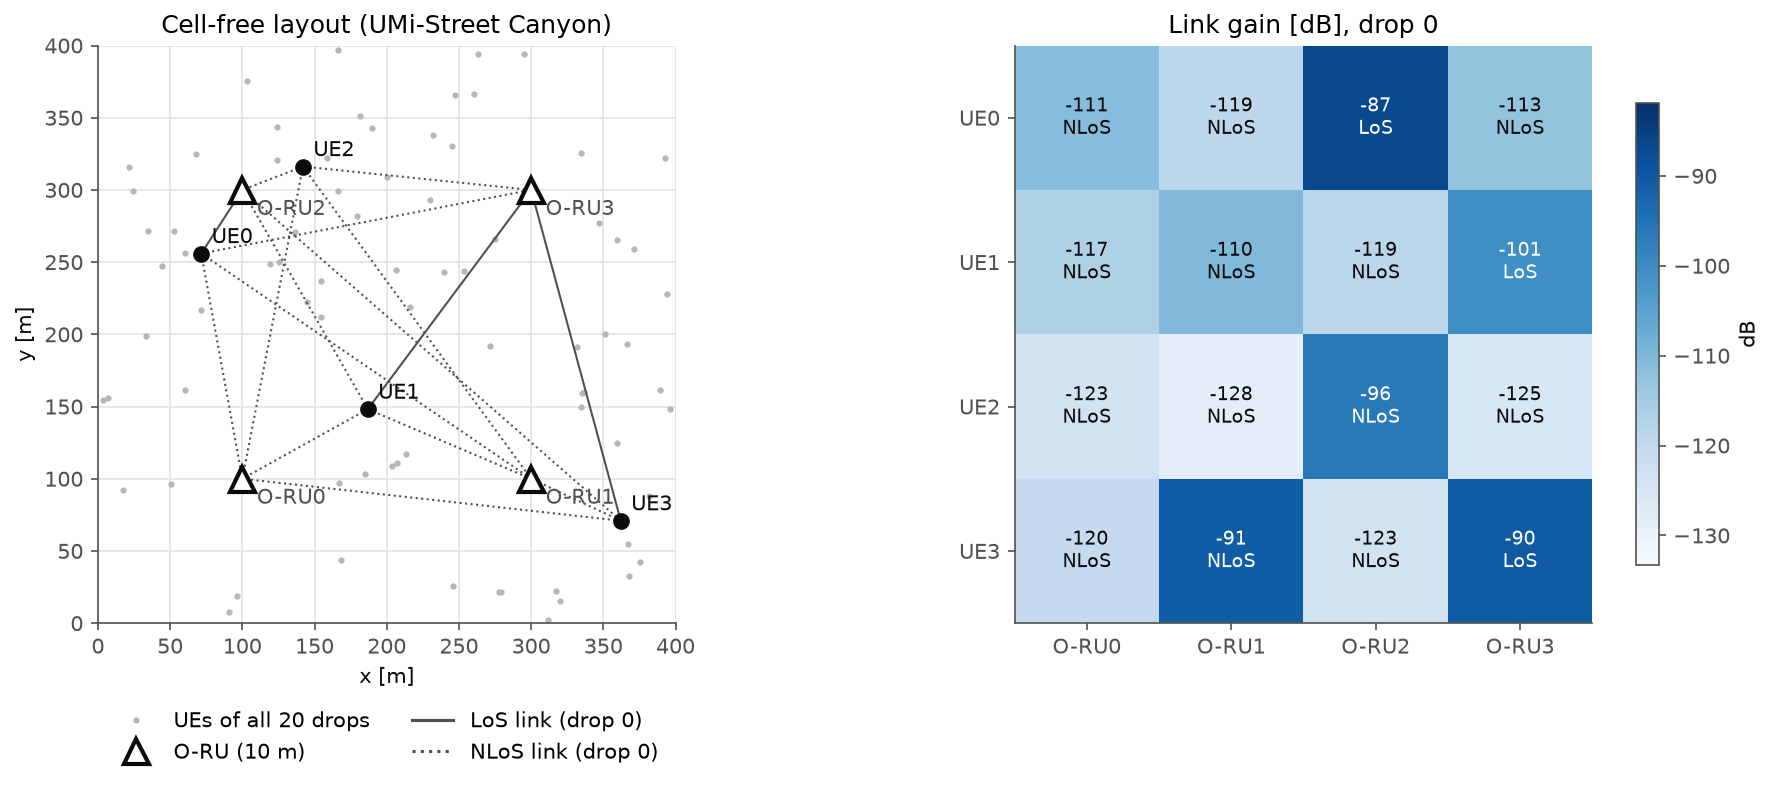
\includegraphics[width=\textwidth]{figures/f1_layout.png}
\caption{F1: cell-free layout. Left: the 4 O-RUs, the 4 UEs of the first drop (solid lines LoS, dotted NLoS) and the UE positions
of all drops (grey). Right: link gain (path loss + shadowing + antennas, averaged over antenna pairs and subcarriers) of every
(UE, O-RU) pair in the first drop.}
\label{fig:f1layout}
\end{figure}

The first drop illustrates the scenario. The wideband SNR per receive antenna of the four UEs is 40.4 / 27.2 / 30.9 / 39.7\dB;
the first-path delays of the O-RUs relative to the UE timing reach about 0.93\,$\mu$s; after the common power scaling the four
O-RUs use 0.017 / 0.32 / 1.0 / 0.68 of their power budget, so O-RU0, which is far from all UEs, transmits about 18\dB below
nominal. This is why \code{fronthaul_agc} is needed: without it the uniform quantizers of 7-1 and option 8 would waste much of
their resolution.

With the ideal fronthaul, the four UEs of a drop together get 390.7\,Mbit/s (20\,MHz), with mean BLER 0.010 and mean MCS 24.7.
54 of the 80 UEs report CQI 15 in all four periods, the others 10--14. The median measured data-slot SINR is 29.1\dB (median
wideband SNR 34.7\dB), mainly limited by residual BD interference within the PRG: the O-RUs have different propagation delays,
and the resulting phase differences within a PRG make the nulls exact only at the centre subcarrier.

\subsection{Results}

\begin{table}[H]
\centering
\caption{F1: fronthaul load and throughput of every split and compression setting (20 drops; per-link loads are for one O-RU
link, ``4 links'' is the sum over all O-RUs)}
\label{tab:f1}
\footnotesize
\setlength{\tabcolsep}{4pt}
\resizebox{\textwidth}{!}{%
\begin{tabular}{@{}l l r r r r r r r r r@{}}
\toprule
 & & \multicolumn{4}{c}{Fronthaul load (Gbit/s)} & Tput & & Mean & & SQNR \\
\cmidrule(lr){3-6}
Split & Compression & link 20\,M & link 100\,M & C-plane & 4 links 100\,M & (\%) & BLER & MCS & $\Delta$CQI & (dB) \\
\midrule
\multirow{4}{*}{option 7-1} & 16 bit & 4.57 & 24.29 & 0     & 97.2  & 100.0 & 0.010 & 24.7 & $+0.00$ & 82.4 \\
                            & 10 bit & 2.92 & 15.21 & 0     & 60.9  & 100.0 & 0.010 & 24.7 & $+0.00$ & 50.8 \\
                            & \textbf{8 bit}  & 2.28 & 12.19 & 0     & \textbf{48.8}  & 99.9  & 0.010 & 24.6 & $-0.00$ & 40.3 \\
                            & 6 bit  & 1.73 &  9.16 & 0     & 36.7  & 98.1  & 0.021 & 24.5 & $-0.10$ & 29.8 \\
\midrule
\multirow{5}{*}{7.2x Cat A} & BFP 9  & 2.67 & 14.35 & 0.008 & 57.4  & 100.0 & 0.010 & 24.7 & $+0.00$ & 49.6 \\
                            & \textbf{BFP 7}  & 2.13 & 11.31 & 0.008 & \textbf{45.2}  & 99.7  & 0.013 & 24.6 & $-0.01$ & 37.6 \\
                            & BFP 5  & 1.58 &  8.16 & 0.008 & 32.6  & 95.0  & 0.038 & 24.0 & $-0.33$ & 25.6 \\
                            & BS 5   & 1.58 &  8.16 & 0.008 & 32.6  & 97.2  & 0.027 & 24.3 & $-0.16$ & 27.9 \\
                            & $\mu$-law 5 & 1.58 & 8.16 & 0.008 & 32.6 & 85.1 & 0.155 & 24.4 & $-0.12$ & 25.1 \\
\midrule
\multirow{7}{*}{7.2x Cat B} & BFP 9  & 1.37 &  7.36 & 0.192 & 29.5  & 100.0 & 0.010 & 24.7 & $+0.00$ & 50.7 \\
                            & BFP 7  & 1.09 &  5.81 & 0.157 & 23.2  & 99.8  & 0.013 & 24.7 & $+0.01$ & 38.6 \\
                            & BFP 5  & 0.81 &  4.20 & 0.122 & 16.8  & 79.2  & 0.215 & 24.5 & $-0.05$ & 27.1 \\
                            & BS 5   & 0.81 &  4.20 & 0.122 & 16.8  & 95.8  & 0.048 & 24.6 & $-0.04$ & 29.0 \\
                            & $\mu$-law 5 & 0.81 & 4.20 & 0.122 & 16.8 & 87.3 & 0.134 & 24.5 & $-0.07$ & 25.0 \\
                            & ModComp / w BFP 9 & 0.59 & 2.97 & 0.216 & 11.9 & 100.0 & 0.010 & 24.7 & $+0.00$ & 74.7 \\
                            & \textbf{ModComp / w BFP 7} & 0.58 & 2.94 & 0.181 & \textbf{11.7} & 100.0 & 0.010 & 24.7 & $+0.00$ & 74.7 \\
\midrule
\multirow{4}{*}{option 8}   & 16 bit & 8.13 & 32.53 & 0     & 130.1 & 100.0 & 0.010 & 24.7 & $+0.00$ & 87.8 \\
                            & 10 bit & 5.09 & 20.38 & 0     & 81.5  & 100.0 & 0.010 & 24.7 & $+0.01$ & 53.7 \\
                            & \textbf{8 bit}  & 4.11 & 16.27 & 0     & \textbf{65.1}  & 100.0 & 0.010 & 24.7 & $+0.00$ & 42.7 \\
                            & 6 bit  & 3.13 & 12.24 & 0     & 49.0  & 98.9  & 0.021 & 24.6 & $-0.02$ & 31.9 \\
\bottomrule
\end{tabular}}

\smallskip
\parbox{\textwidth}{\footnotesize Throughput relative to the ideal fronthaul on the same drops; $\Delta$CQI relative to the CQI with
ideal fronthaul; BS = block scaling; ModComp / w BFP $x$ = modulation compression with BFP $x$-bit weights. Bold: cheapest
configuration of each split with throughput $\ge 99\%$. The modulation-compression load is computed from the actual MCS of each
period and averaged.}
\end{table}

\begin{table}[H]
\centering
\caption{F1: lowest fronthaul load per split with throughput $\ge 99\%$ of the ideal fronthaul (100\,MHz)}
\label{tab:f1best}
\footnotesize
\begin{tabular}{@{}l l r r r@{}}
\toprule
Split & Operating point & 4 links (Gbit/s) & per link (Gbit/s) & Throughput \\
\midrule
option 7-1 & 8-bit fixed point                   & 48.8 & 12.2 & 99.9\% \\
7.2x Cat A & BFP 7                                       & 45.2 & 11.3 & 99.7\% \\
7.2x Cat B & ModComp + BFP 7 weights      & 11.7 & 2.9 (C-plane 0.18) & 100\% \\
option 8   & 8-bit fixed point                   & 65.1 & 16.3 & 100\% (6 bit: 98.9\%) \\
\bottomrule
\end{tabular}
\end{table}

\begin{figure}[H]
\centering
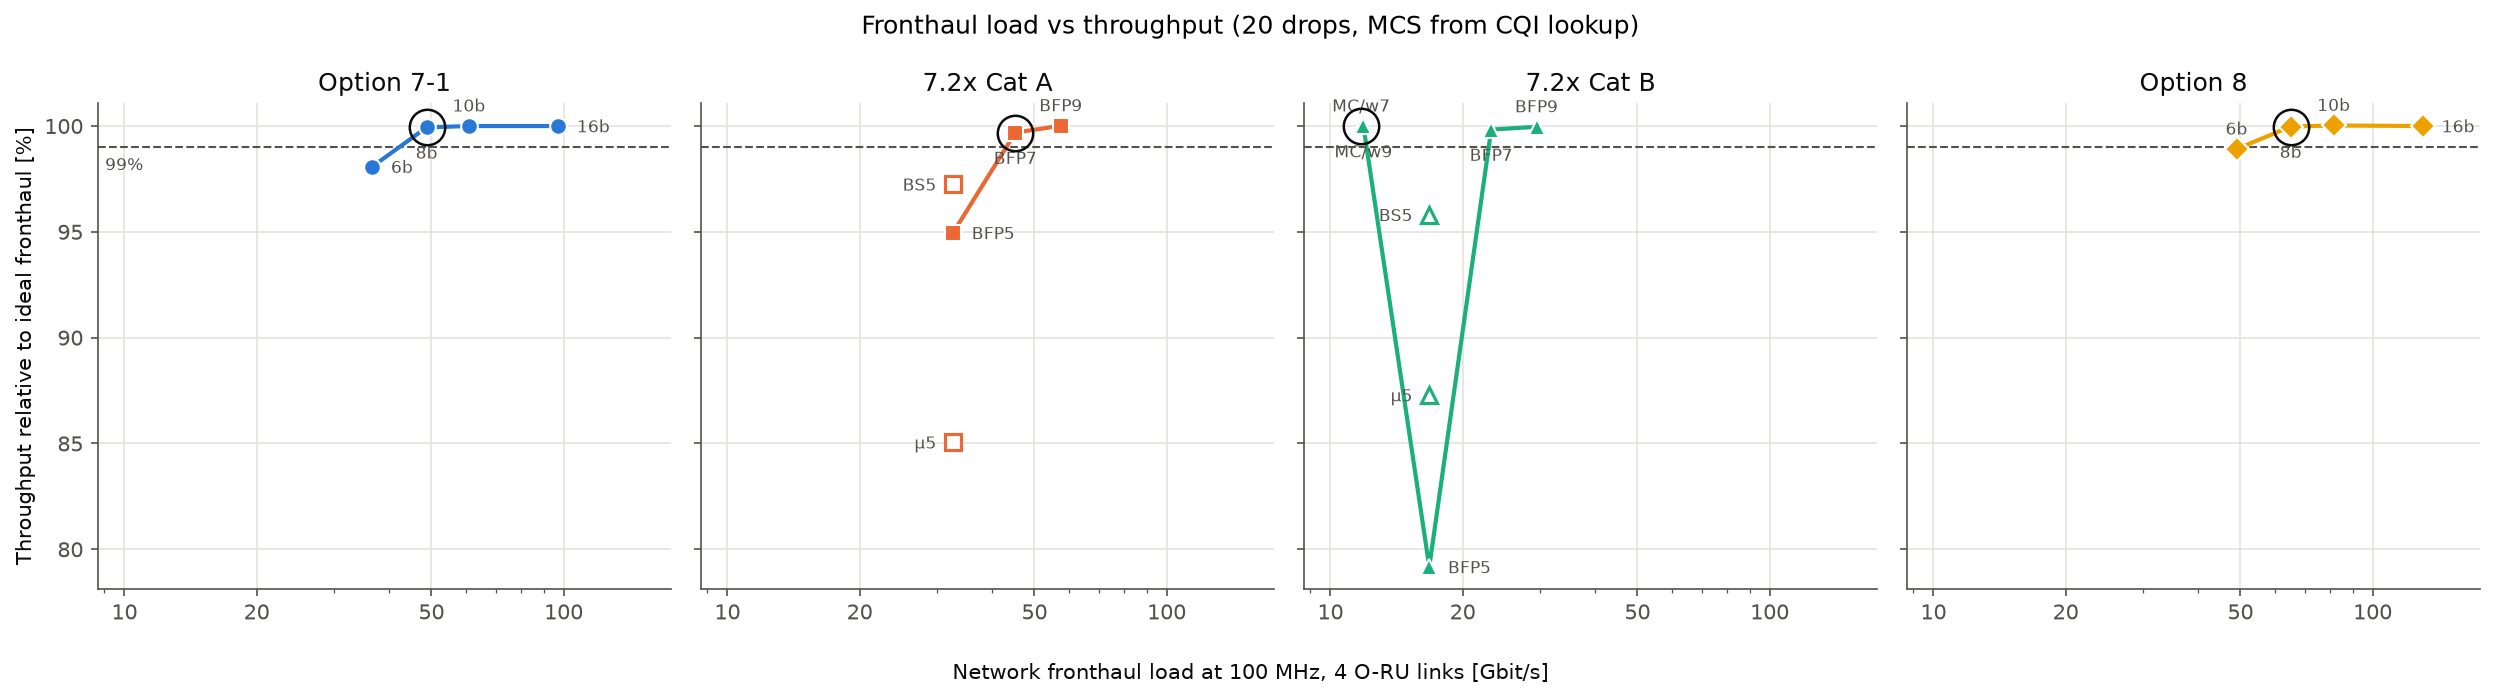
\includegraphics[width=\textwidth]{figures/f1_load_vs_throughput.png}
\caption{F1: network fronthaul load (100\,MHz, sum of 4 O-RU links, log scale) versus relative throughput, one panel per split.
Filled markers: uniform fixed point (7-1, 8), BFP and modulation compression (Cat A / B); hollow markers: block scaling (BS) and
$\mu$-law at the same number of bits; ring: operating point (cheapest configuration with throughput $\ge 99\%$); dashed line:
99\%. ``MC/w7'' is modulation compression with BFP 7 weights.}
\label{fig:f1load}
\end{figure}

\begin{figure}[H]
\centering
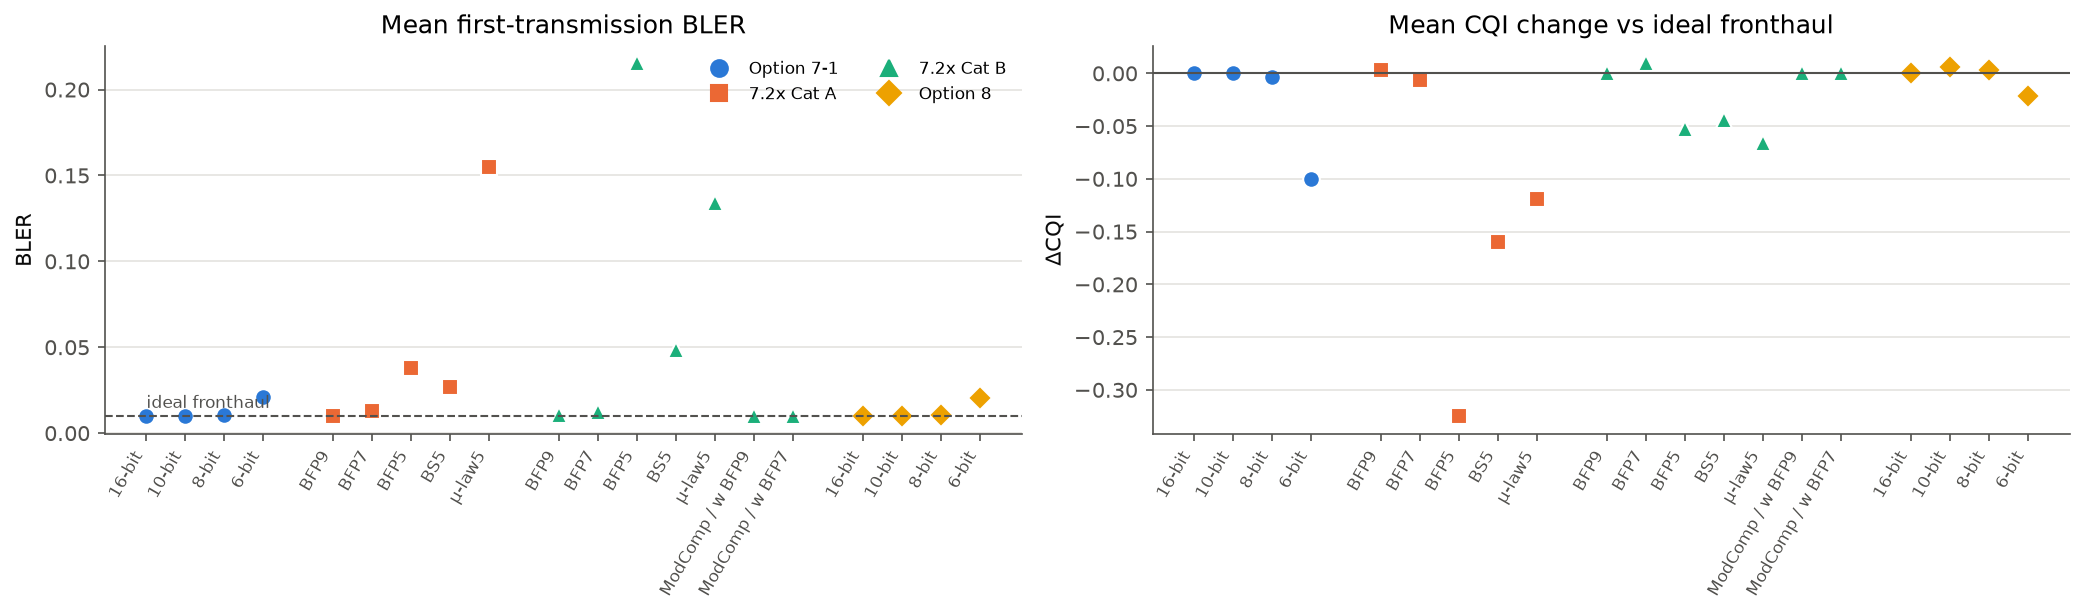
\includegraphics[width=\textwidth]{figures/f1_bler_dcqi.png}
\caption{F1: where the throughput goes. Left: mean first-transmission BLER (distortion the CQI did not see turns into block
errors). Right: mean CQI change relative to the ideal fronthaul (distortion the CQI did see lowers the MCS).}
\label{fig:f1diag}
\end{figure}

\begin{figure}[H]
\centering
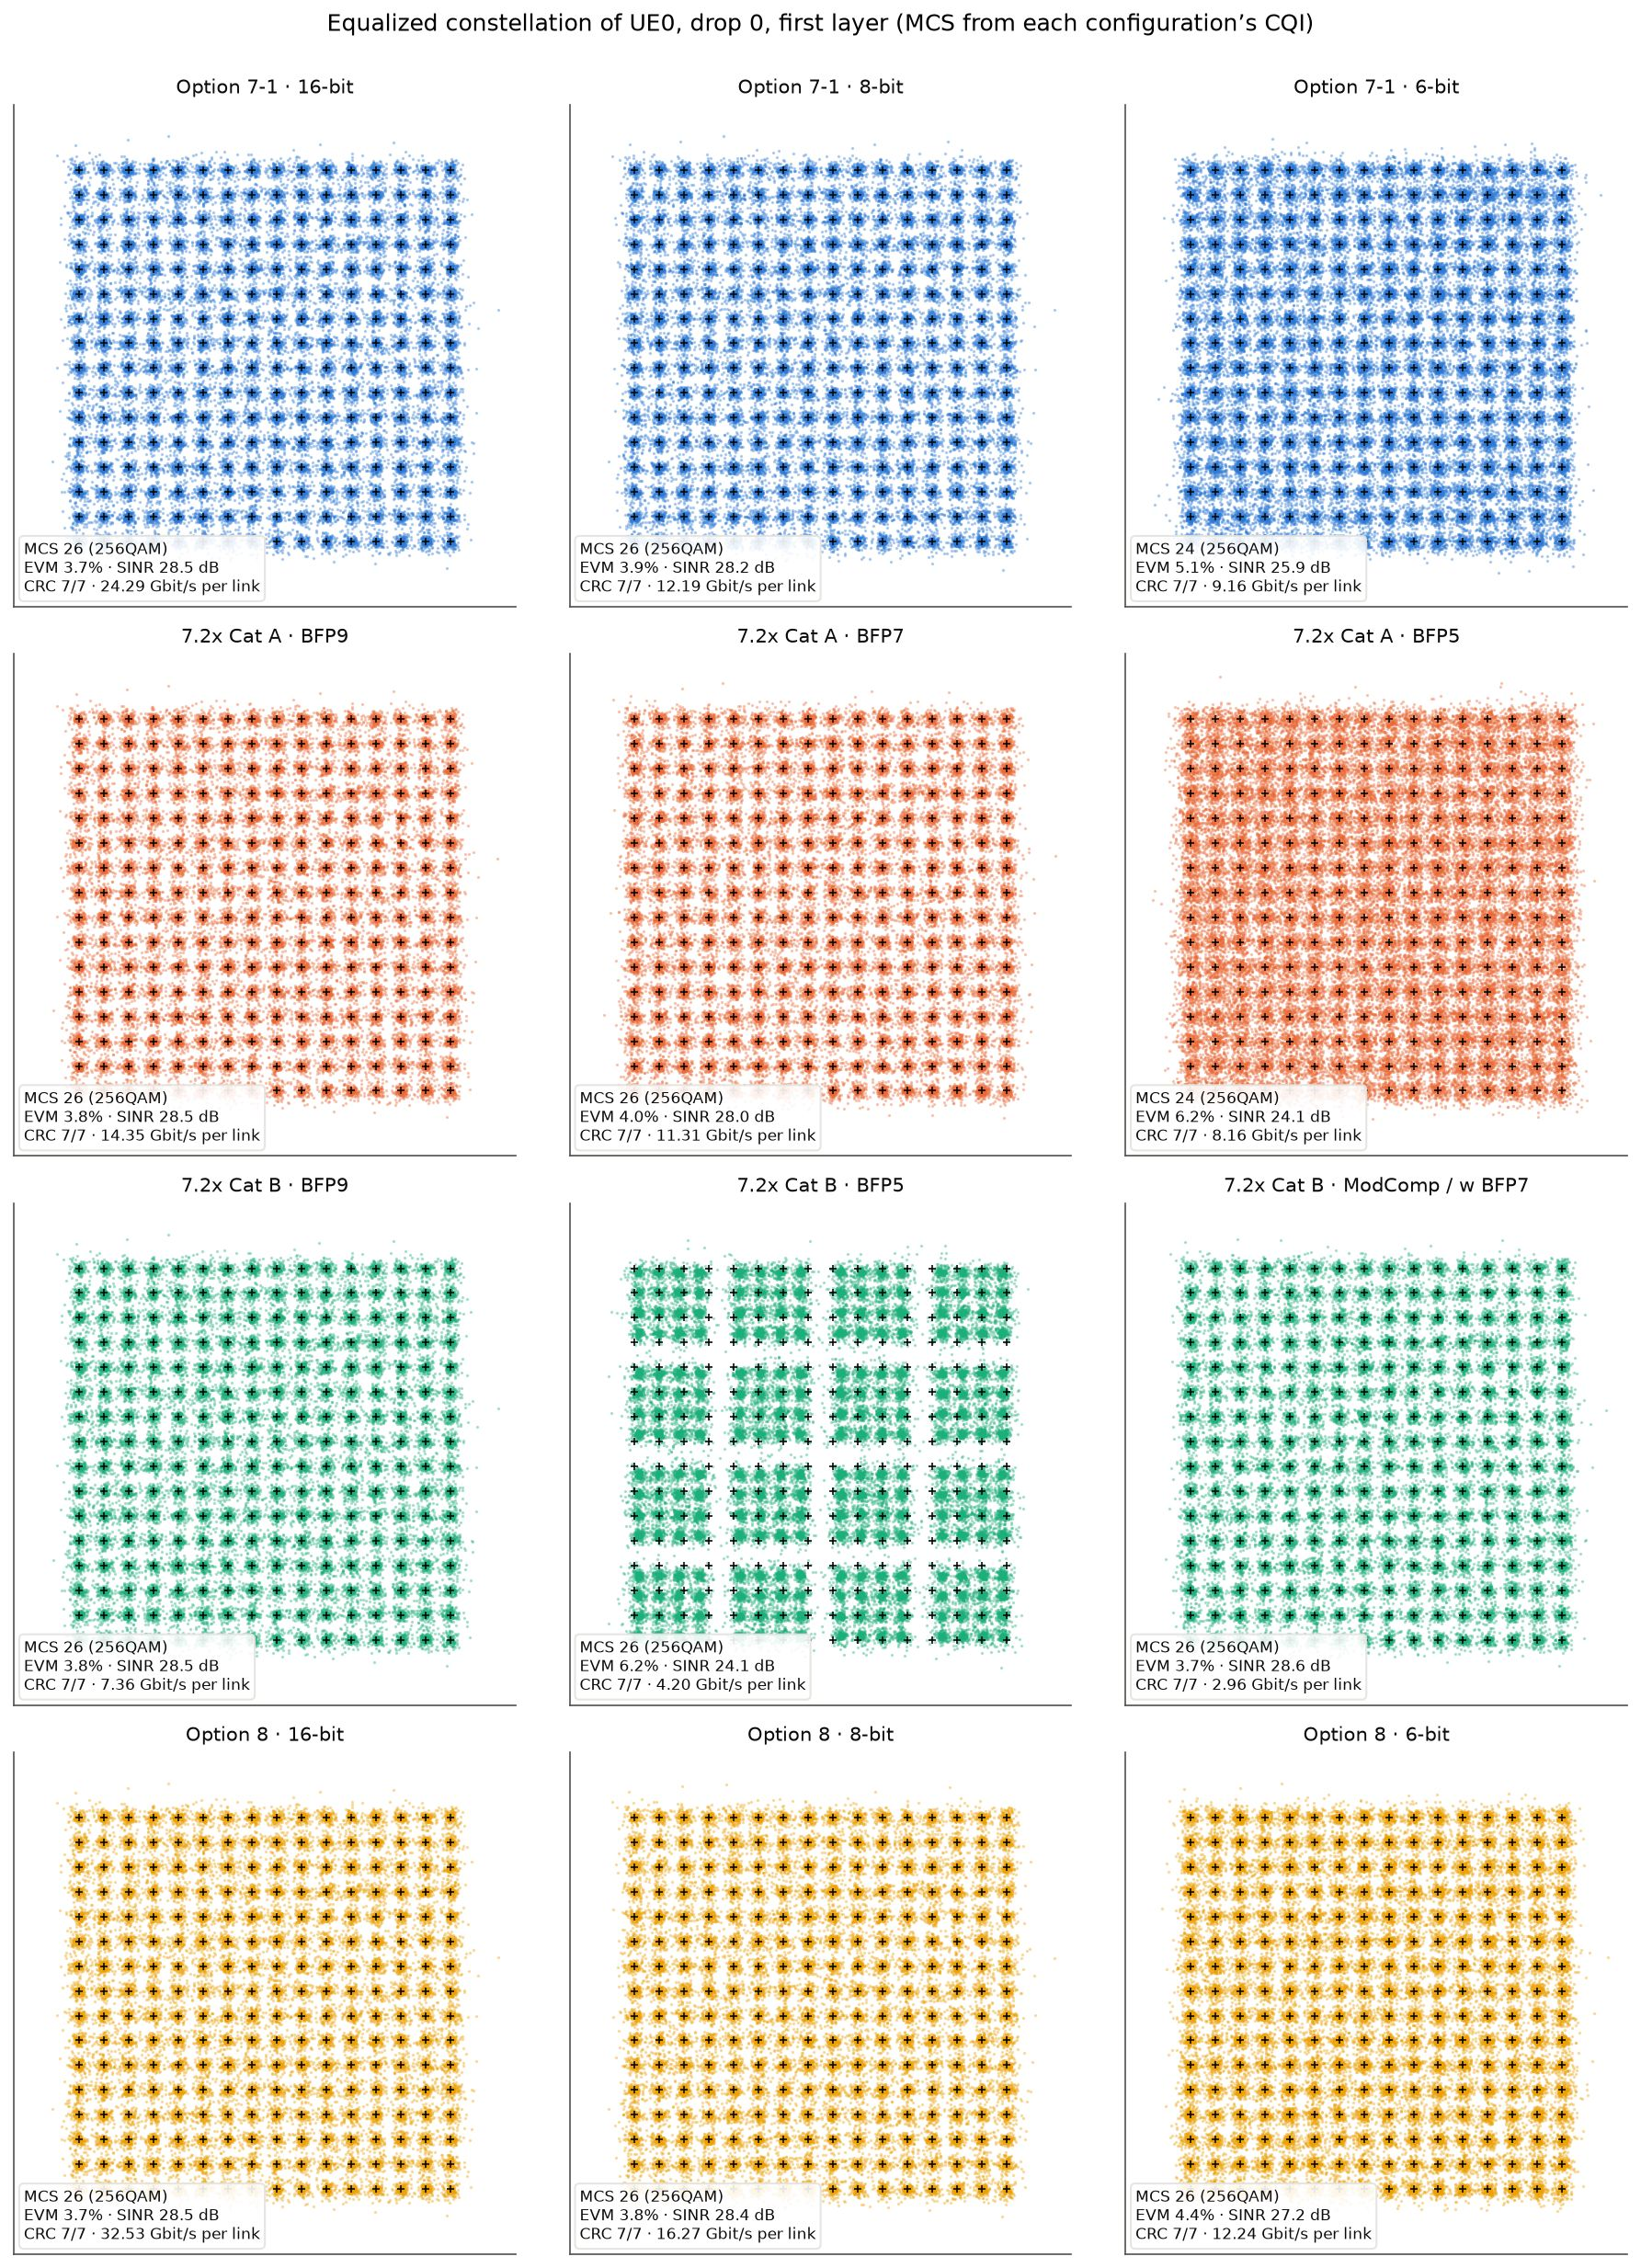
\includegraphics[width=0.86\textwidth]{figures/f1_constellations.jpg}
\caption{F1: equalized constellation of UE0's first layer in drop 0 (MCS from each configuration's own CQI; crosses are the ideal
constellation points). One row per split, one column per compression setting; the boxes give the MCS, the EVM and corresponding
SINR, the CRC results of the 7 slots, and the per-link load at 100\,MHz. With Cat B BFP 5 the points are pulled onto the
quantizer grid in blocks (a deterministic displacement); modulation compression keeps the points intact.}
\label{fig:f1const}
\end{figure}

\begin{figure}[H]
\centering
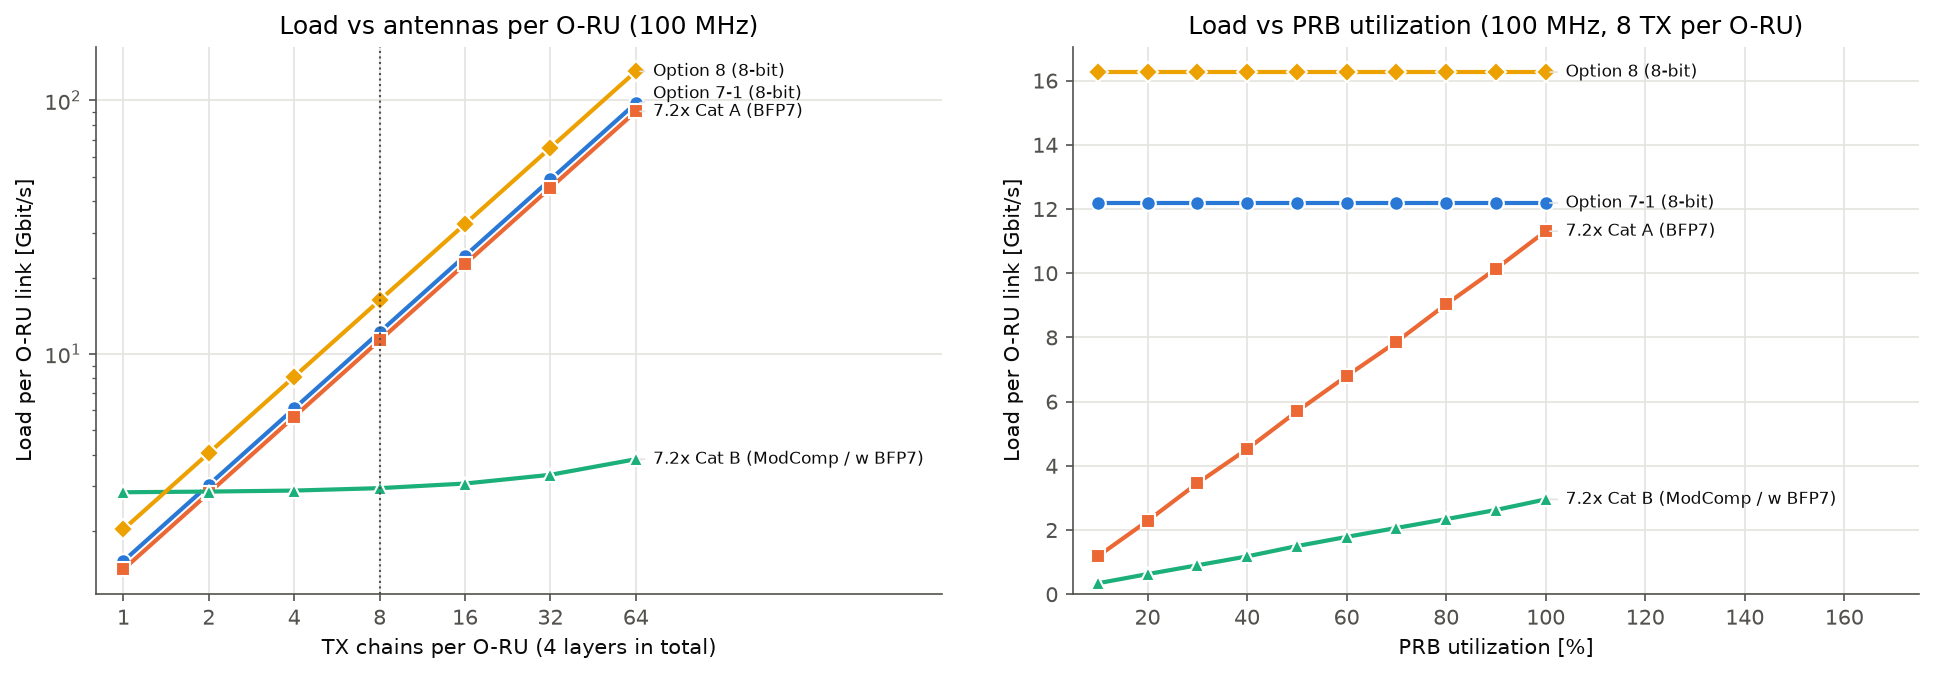
\includegraphics[width=\textwidth]{figures/f1_load_scaling.png}
\caption{F1: analytic per-link load (100\,MHz) at each split's operating point (Table~\ref{tab:f1best}). Left: versus TX chains
per O-RU (4 layers in total; Cat B modulation compression assumes worst-case 256QAM). Right: versus PRB utilization (8 TX per
O-RU).}
\label{fig:f1scaling}
\end{figure}

\subsection{Analysis}

\begin{enumerate}
  \item \textbf{Cat B with modulation compression needs about a quarter of the load of the other splits, without loss}
        (11.7 vs 45--65\Gbps). There are two reasons: each O-RU receives 4 layers instead of 8 antenna streams, and each RE needs
        only $Q_m$ bit (8 bit for 256QAM) instead of about 15--16 bit. The load follows the MCS, but since most UEs use 256QAM in
        this scenario, each link stays between 2.79 and 2.96\Gbps (BFP 7 weights). Without modulation compression, Cat B needs
        23.2\Gbps at BFP 7 (99.8\%), and at BFP 5 its throughput falls to 79\%.
  \item \textbf{7-1 and Cat A are almost equal at full load.} 8-bit uniform fixed point is 16 bit/RE, BFP 7 is
        $(24\times7+8)/12 = 14.7$ bit/RE plus headers; the difference is only the compression method. The real drawback of 7-1
        concerns scheduling: at low PRB utilization the Cat A load falls proportionally, while 7-1 stays constant
        (Figure~\ref{fig:f1scaling}, right).
  \item \textbf{Option 8 needs about one third more than 7-1 at the same width (100\,MHz).} Option 8 carries 122.88\,Msps per
        antenna (4096-point IFFT, including guard band and CP), while 7-1 carries $3276 \times 28000 = 91.7$\,M RE/s; at 20\,MHz the
        ratio is $30.72/17.14 = 1.8$. On the other hand, the time-domain quantization noise is spread over all IFFT bins and only
        612/1024 of it falls in band, so in the 20\,MHz simulation the in-band SQNR is about 2.2\dB higher than 7-1 at the same width
        (8 bit: 42.7 vs 40.3\dB), and the loss at 6 bit is smaller (98.9\% vs 98.1\%). At 100\,MHz this advantage shrinks to
        $10\log_{10}(4096/3276) \approx 1$\dB.
  \item \textbf{5 bit is the breaking point, and the CSI-RS hardly sees it.} F1 uses pure table lookup without OLLA, so distortion
        the CQI misses turns directly into block errors:
        \begin{itemize}
          \item Cat B BFP 5: BLER 0.215 with $\Delta$CQI of only $-0.05$. The layer symbols themselves are quantized; the 5-bit BFP
                step (about 0.12 for unit-power 256QAM) is comparable to the 256QAM point spacing (about 0.15), so the points are
                pulled onto the quantizer grid in blocks (Figure~\ref{fig:f1const}) and the error is deterministic;
          \item Cat A BFP 5: BLER 0.038 with $\Delta$CQI $-0.33$. The co-scheduled UEs' distortion enters the CQI through the
                NZP-IMR, so the MCS is lowered somewhat;
          \item among the 5-bit methods, $\mu$-law is the worst in Cat A (85\% throughput) and block scaling the best (97\% / 96\%),
                at the same number of bits.
        \end{itemize}
  \item \textbf{The throughput loss is concentrated on UEs below the top MCS.} Table~\ref{tab:f1ue} splits the UEs into those
        that report CQI 15 in all four periods with the ideal fronthaul (54 UEs) and the rest (26 UEs). The CQI-15 UEs have SINR
        to spare above that CQI's threshold; the others sit right at the threshold of the selected MCS and fail as soon as
        distortion is added.
  \item \textbf{Scaling with antennas and utilization} (Figure~\ref{fig:f1scaling}). 7-1, Cat A and option 8 grow linearly with
        the number of TX chains per O-RU; Cat B grows with the number of layers, plus weights that grow slowly with the antennas
        (2.96\Gbps at 8 TX, 3.84\Gbps at 64 TX). With only 1--2 TX chains per O-RU, Cat B has no advantage (1 TX: Cat A 1.41 vs
        Cat B 2.85\Gbps; 2 TX: about equal, 2.83 vs 2.86), because every O-RU must receive all 4 layers. The more antennas per
        O-RU, the larger the Cat B advantage.
  \item \textbf{Cross-check.} For 7-1 with 8 antennas, 2$\times$16 bit and 100\,MHz, this model gives 24.3\Gbps and the TR 38.816
        formula 21.5\Gbps; the reasons are given in Section~\ref{sec:load}.
\end{enumerate}

\begin{table}[H]
\centering
\caption{F1: mean first-transmission BLER per UE class (``CQI 15'': the 54 UEs that report CQI 15 in all four periods with the
ideal fronthaul; ``others'': the remaining 26)}
\label{tab:f1ue}
\footnotesize
\begin{tabular}{@{}l l r r@{}}
\toprule
Split & Compression & CQI-15 UEs & Others \\
\midrule
option 7-1 & 6 bit             & 0.001 & 0.063 \\
option 8   & 6 bit             & 0.000 & 0.063 \\
7.2x Cat A & BFP 5             & 0.005 & 0.106 \\
7.2x Cat A & block scaling 5   & 0.006 & 0.070 \\
7.2x Cat A & $\mu$-law 5       & 0.128 & 0.212 \\
7.2x Cat B & BFP 5             & 0.172 & 0.305 \\
7.2x Cat B & block scaling 5   & 0.028 & 0.089 \\
7.2x Cat B & $\mu$-law 5       & 0.097 & 0.212 \\
\bottomrule
\end{tabular}
\end{table}

Cat B BFP 5 and both 5-bit $\mu$-law settings cause errors even for the CQI-15 UEs, i.e.\ their distortion exceeds the margin of
the top MCS; for the other settings almost all block errors come from UEs near a threshold.

% =====================================================================
\section{Discussion}
% =====================================================================

\subsection{Answers to the three questions}

\begin{description}[leftmargin=1.2em, style=nextline]
  \item[Q1] In the open loop, BFP at 9 and 7 bit is practically lossless for 256QAM, 6 bit starts to cost, 5 bit is the breaking
        point and 4 bit is unusable. With two-user BD, Cat A is more sensitive than Cat B (antenna-domain noise cannot be nulled
        by BD). At equal width block scaling beats BFP and $\mu$-law (2.0--5.6\dB more SQNR), but in Cat B the SQNR does not
        fully predict the loss.
  \item[Q2] The CSI-IM never sees compression distortion. With one user the CSI-RS does not see it either (self-distortion only
        appears as channel-estimation error). With two users the NZP-IMR sees the co-scheduled UE's leaked distortion and the null
        errors caused by weight compression, 30--45\% of the data-slot SINR drop. The rest (self-distortion) appears as a
        negative OLLA offset in the closed loop, or directly as block errors without OLLA (F1).
  \item[Q3] See Table~\ref{tab:f1best}: the lowest lossless load is 45--65\Gbps for 7-1, Cat A and option 8 (4 links, 100\,MHz) and
        11.7\Gbps for Cat B with modulation compression. The Cat B advantage grows with the antennas per O-RU; the Cat A load
        falls with PRB utilization, whereas 7-1 and option 8 do not depend on scheduling.
\end{description}

\subsection{Patterns across the experiments}

\begin{itemize}
  \item \textbf{Where the distortion enters matters more than how large it is.} Antenna-domain distortion (Cat A, 7-1, 8) leaks to
        co-scheduled UEs in MU; layer-domain distortion (Cat B) hurts only its own UE but gets the same beamforming gain as the
        signal. Hence Cat B is more sensitive with SU and Cat A with MU.
  \item \textbf{The CSI only sees other users' distortion.} Only cross-user distortion measured on the NZP-IMR enters the CQI;
        self-distortion is invisible to the CSI. Link adaptation has to rely on OLLA or on a distortion-aware CQI
        (Section~\ref{sec:future}).
  \item \textbf{Margin decides the cost.} High-SNR UEs sit at the top MCS and distortion only eats their margin; the throughput
        loss is concentrated on UEs whose SINR is right at a threshold. The mean SINR drop therefore greatly overstates the
        throughput loss, and compression schemes should be judged by closed-loop throughput.
  \item \textbf{5 bit is the common breaking point} in all settings, and BFP at 7 bit is safe in all of them (throughput loss
        $\le 4\%$, mostly $< 0.5\%$).
\end{itemize}

\subsection{Baseline settings for later directions}

\begin{table}[H]
\centering
\caption{Recommended baseline (defaults of \code{oran/config.py} and the settings of this direction's scripts)}
\label{tab:baseline}
\footnotesize
\begin{tabularx}{\textwidth}{@{}P{3.0cm} Y@{}}
\toprule
Item & Baseline \\
\midrule
Carrier & simulate 30\,kHz SCS, 51 PRBs (20\,MHz); report loads scaled to 273 PRBs (100\,MHz) \\
MCS / CQI & MCS table 2 and CQI table 2 (up to 256QAM); MCS 20 for open-loop comparisons; usable MCS 3--27 \\
Default fronthaul & U-plane BFP 9 bit, Cat B weights BFP 9 bit (indistinguishable from the ideal fronthaul); BFP 7 bit as the
                    ``lowest lossless width'' reference \\
Precoding & BD, PRG 2 PRBs, ideal CSI (TDD reciprocity) \\
Closed loop & CQI from CSI-RS / CSI-IM through the fronthaul (\code{cqi_source="csi-rs"}), genie CQI always recorded for comparison;
              CSI-RS period = 1 measurement + 7 data slots; OLLA step 0.5\dB, BLER target 0.1; 16 periods per drop, first 4
              excluded \\
Channel & single-cell closed loop: Sionna RT munich scene, O-RU at 35\,dBm; cell-free: TR 38.901 UMi grid with per-O-RU power
          limit and fronthaul AGC \\
Statistics & paired comparisons: run all configurations on the same drop with the same seed; across processes share a drop file
             and use \code{CUDA_VISIBLE_DEVICES} so that every process sees the same device index \\
\bottomrule
\end{tabularx}
\end{table}

% =====================================================================
\section{Limitations and future work}
\label{sec:future}
% =====================================================================

\paragraph{Limitations.}
\begin{itemize}
  \item Full buffer, all PRBs scheduled, static UEs; no HARQ (first transmissions only); CSI reports without errors or delay;
        fixed rank, no RI adaptation.
  \item Precoding uses ideal CSI. BD nulls only at the PRG centre subcarrier, and at high SNR the residual interference often
        caps the SINR, which hides part of the fronthaul distortion.
  \item E2's CQI is an ideal measurement (it ran before the CSI-RS existed). In E1 the Cat B weights are fixed at BFP 9, whereas in
        E3 and F1 they use the same width as the U-plane; keep this in mind when comparing Cat B across experiments.
  \item F1 assumes full cooperation (every UE served by every O-RU), with no user-centric serving clusters; only outdoor UEs (80\%
        are indoor in TR 38.901 Table 7.2-1); one layer per UE; pure CQI lookup. The 100\,MHz loads scale the 20\,MHz configuration
        to 273 PRBs; the throughput criterion comes from the 20\,MHz simulation.
  \item The load model ignores CPRI line coding and control words for option 8; the C-plane overhead of modulation compression is
        estimated from the formats; selective RE sending (Annex A.6) is not implemented.
  \item The number of drops is limited (30 in E2 / E3, 20 in F1), so tail statistics such as the 5th percentile are uncertain.
  \item \code{closed_loop_walkthrough.ipynb} was re-run on a laptop whose GPU intermittently misreads memory (RTX 4060 Laptop, found
        on 29 October 2026), and the repository README asks for its outputs to be re-checked. No statistical conclusion of this
        report comes from that notebook. E1--E3 ran on the T4 server and F1 on a T4, and are not affected.
\end{itemize}

\paragraph{Future work.}
\begin{itemize}
  \item User-centric serving clusters (each UE served by a subset of O-RUs): the load then varies per drop, and in Cat B each
        O-RU only needs the layers of the UEs in its clusters.
  \item Monte Carlo verification of partial PRB utilization (only analytic so far); two layers per UE (needs double-symbol DMRS).
  \item Distortion-aware CQI: TS 38.214 \S 5.2.1.4.1 allows the UE to include ``other interference'' on the CMR REs in the CQI.
        A 2-port, density-1 CMR has only 2 REs per PRB, which leaves no degrees of freedom to separate distortion from the channel;
        denser measurement resources or TRS / DMRS residuals would be needed.
  \item Generate and decode the measurement-slot PDSCH with rate matching; RI adaptation; HARQ (redundancy versions + soft
        combining); UE mobility (Doppler on ray-traced paths) and CSI report delay.
  \item Selective RE sending (Annex A.6) combined with modulation compression, to remove the bits spent on empty REs.
\end{itemize}

% =====================================================================
\appendix
\section{How to reproduce}
% =====================================================================

All scripts run from the repository root. Activate the environment first (the path contains a space and must be quoted):
\begin{lstlisting}
cd "/home/user/Sionna-based Simulation"
source env.sh
python -m unittest discover -s tests -v          # unit tests, about 45 s
\end{lstlisting}

\paragraph{E1 / E1$'$: open-loop Cat A / B comparison.}
\begin{lstlisting}
# BFP width sweep: one category per GPU (both mapped to cuda:0 so the random draws are identical), then merge
CUDA_VISIBLE_DEVICES=0 python studies/oran_baseline/compare_cat_a_b.py --categories A --out results/cat_a &
CUDA_VISIBLE_DEVICES=1 python studies/oran_baseline/compare_cat_a_b.py --categories B --out results/cat_b &
wait
python studies/oran_baseline/compare_cat_a_b.py --merge results/cat_a results/cat_b --out results/cat_ab

# Compression methods (E1')
python studies/oran_baseline/compare_cat_a_b.py --categories A \
    --widths ideal 6 bs:6 mu:6 5 bs:5 mu:5 bs:4 --out results/methods_a
# Cat B likewise (--categories B --out results/methods_b), then --merge into results/methods
\end{lstlisting}
Values of \code{--widths}: \code{ideal} (ideal fronthaul), \code{none16} (16-bit uncompressed), an integer $w$ (BFP), or
``method:$w$'' with method \code{bfp}, \code{bs} or \code{mu}. \code{--bfw-width} sets the Cat B weights (default 9; \code{same}
means the same as the U-plane).

\paragraph{E2: ray-traced closed-loop baseline.}
\begin{lstlisting}
python studies/oran_baseline/rt_closed_loop.py --num-ue 1                  # SU, results in results/rt_su
python studies/oran_baseline/rt_closed_loop.py --num-ue 2                  # MU, results in results/rt_mu
python studies/oran_baseline/rt_closed_loop.py --cqi-source genie          # reference: genie CQI
python studies/oran_baseline/rt_closed_loop.py --replot results/rt_su      # re-plot only
\end{lstlisting}
Note: the current script defaults to \code{--cqi-source csi-rs} and \code{--batch-size 7}. To approximate the conditions of E2 use
\code{--cqi-source genie --batch-size 8} (still not identical, since E2 had no measurement slot).

\paragraph{E3: visibility of compression distortion.}
\begin{lstlisting}
python studies/oran_baseline/rt_compare_compression.py --num-ue 2 --save-drops results/drops_mu.json
CUDA_VISIBLE_DEVICES=0 python studies/oran_baseline/rt_compare_compression.py --num-ue 2 \
    --categories A --drops-file results/drops_mu.json --out results/csi_mu_a &
CUDA_VISIBLE_DEVICES=1 python studies/oran_baseline/rt_compare_compression.py --num-ue 2 \
    --categories B --drops-file results/drops_mu.json --out results/csi_mu_b &
wait
python studies/oran_baseline/rt_compare_compression.py --merge results/csi_mu_a results/csi_mu_b --out results/csi_mu
# SU: --num-ue 1, drop file results/drops_su.json, outputs csi_su_a / csi_su_b / csi_su
\end{lstlisting}

\paragraph{F1: four splits in cell-free MIMO.} Run \code{studies/oran_baseline/split_fronthaul_load.ipynb} in VS Code
(\code{NUM_DROPS = 20}, \code{SEED = 2026}). With \code{SAVE_RESULTS = True} the results go to
\code{results/split_fronthaul_load_<date>/run_<time>_drops<N>_seed<S>/}: \code{metadata.json}, a source snapshot, per-row results
\code{rows.jsonl}, \code{complete.json} with the summary, and \code{fig_*.png}.

\paragraph{This report.} \code{python studies/oran_baseline/report/make_figures.py} re-plots the E1--E3 figures with English labels
from the stored \code{results.json} files (no simulation) and copies the F1 figures; then run \code{latexmk} in
\code{studies/oran_baseline/report/}.

\section{Files and result directories}

\begin{table}[H]
\centering
\caption{Files in \code{studies/oran_baseline/}}
\footnotesize
\begin{tabularx}{\textwidth}{@{}l l Y@{}}
\toprule
File & Type & Content \\
\midrule
\code{compare_cat_a_b.py} & run + summary & Cat A/B $\times$ compression width $\times$ SNR sweep (E1 / E1$'$); can run per GPU and \code{--merge} \\
\code{rt_closed_loop.py} & run & ray-traced closed loop: drop $\to$ CSI-RS $\to$ CQI $\to$ MCS (+ OLLA) $\to$ PDSCH $\to$ CRC (E2) \\
\code{rt_compare_compression.py} & run + summary & Cat A/B compression distortion in the closed loop, paired drops (E3) \\
\code{split_fronthaul_load.ipynb} & run + summary & four splits $\times$ compression in cell-free MIMO: load, throughput, constellations, load scaling (F1) \\
\code{closed_loop_walkthrough.ipynb} & demo & module-by-module closed-loop walkthrough (Appendix~\ref{sec:walkthrough}) \\
\code{experiments.md} & index & register of experiments from November 2026 on \\
\code{report/} & report & this report (\code{main.tex}, \code{make_figures.py}, \code{figures/}) \\
\bottomrule
\end{tabularx}
\end{table}

\begin{table}[H]
\centering
\caption{Result directories (under \code{results/} in the repository root)}
\footnotesize
\begin{tabularx}{\textwidth}{@{}l Y@{}}
\toprule
Directory & Content \\
\midrule
\code{cat_a}, \code{cat_b}, \code{cat_ab} & E1: \code{results.json}, \code{bler.png}, \code{evm.png}, \code{tradeoff.png}; \code{*.log} are run logs \\
\code{methods_a}, \code{methods_b}, \code{methods} & E1$'$: as above \\
\code{rt_su}, \code{rt_mu} & E2: \code{results.json} (with per-batch CQI, MCS, OLLA, block errors), \code{map.png}, \code{cdf.png}, \code{snr.png}, \code{olla.png} \\
\code{csi_su*}, \code{csi_mu*}, \code{drops_*.json} & E3: \code{results.json}, \code{summary.png}, \code{cdf.png}, \code{gap.png}; \code{drops_*.json} are the drops shared by both GPUs \\
\code{split_fronthaul_load_20261105/run_115332_drops20_seed2026/} & F1 main run (420 rows = 20 drops $\times$ 21 configurations); \code{run_121140_...} is a re-run with identical \code{rows.jsonl} \\
\bottomrule
\end{tabularx}
\end{table}

All numbers in this report were re-aggregated from the \code{results.json} files, logs and \code{complete.json} / \code{rows.jsonl}
of these directories.

\section{The walkthrough notebook}
\label{sec:walkthrough}

\code{closed_loop_walkthrough.ipynb} takes one closed-loop simulation apart along the signal flow. Each step calls the components
in \code{oran/} directly and plots the intermediate results:

\begin{table}[H]
\centering
\footnotesize
\begin{tabularx}{\textwidth}{@{}l Y l@{}}
\toprule
Section & Content & Code \\
\midrule
0--1 & switches and initialization (channel, Cat A/B, compression, SU/MU, CQI source) & \code{config.py} \\
2 & physical environment and channel: 3D scene and paths, power delay profile, frequency response & \code{rt_channel.py}, \code{channel.py} \\
3 & resource grid: PDSCH, DMRS, CSI-RS / CSI-IM & \code{pdsch.py}, \code{csi_rs.py} \\
4 & precoding: per-layer received power after BD, residual interference within the PRG & \code{precoding.py} \\
5 & measurement slot and CQI: CSI-IM noise, NZP-IMR interference, CSI-RS vs genie CQI & \code{csi_rs.py}, \code{csi.py} \\
6 & link adaptation: CQI $\to$ SINR estimate + OLLA $\to$ MCS $\to$ TBS & \code{link_adaptation.py} \\
7 & data slots: O-DU coding chain $\to$ fronthaul (SQNR, load) $\to$ O-RU (TX EVM) $\to$ channel and UE (estimation NMSE, CRC) & \code{odu.py} etc. \\
8 & closed loop over several CSI-RS periods, OLLA convergence & simplified \code{closed_loop.py} \\
9 & Cat A/B $\times$ compression on the same drop (optional) & simplified \code{rt_compare_compression.py} \\
\bottomrule
\end{tabularx}
\end{table}

Results from a single drop are highly random; statistical conclusions should be taken from the batch runs of E2, E3 and F1. See
also the note on re-checking this notebook in Section~\ref{sec:future}.

\end{document}
